\documentclass[a4paper, 14pt]{article}
\usepackage[margin=2.25cm]{geometry}
\usepackage[utf8]{inputenc}
\usepackage{minted}
\usepackage[russian]{babel}
\usepackage{amsmath}
\usepackage{graphicx}
\usepackage{changepage}
\usepackage{hyperref}
\usepackage{cases}
\usepackage{indentfirst}
\usepackage{multirow}
\usepackage{longtable}
\pagestyle{plain}

\hypersetup{
	linkbordercolor = {1 1 1}
}

\usepackage[usenames,dvipsnames,svgnames,table]{xcolor}
\usepackage{tikz-timing}[2009/05/15]
\usepackage{multicol}
\usepackage[T2A]{fontenc}
\usepackage{pgfplots}
\usepackage{pgfgantt}

\usepackage{listings}
\usepackage{caption}
\DeclareCaptionFont{white}{\color{white}} % Текст заголовка.
\DeclareCaptionFormat{listing}{\colorbox{gray}{\parbox{\textwidth}{#1#2#3}}}
\captionsetup[lstlisting]{format=listing,labelfont=white,textfont=white}
\renewcommand\labelenumi{\theenumi)}

\usepackage[backend=biber]{biblatex}
\addbibresource{mybib.bib}

\def\Year{\expandafter\YEAR\the\year}
\def\YEAR#1#2#3#4{#1#2#3#4}

\newcommand{\rusdate}{%
  \ifnum\day<10 0\fi\number\day.%
  \ifnum\month<10 0\fi\number\month.%
  \number\year}


\begin{document}
\lstset{
	language=java,                 % Выбор языка для подсветки (здесь это java).
	basicstyle=\small\sffamily,    % Размер и начертание шрифта для подсветки кода.
	numbers=left,                  % Где поставить нумерацию строк (слева\справа).
	numberstyle=\tiny,             % Размер шрифта для номеров строк.
	stepnumber=1,                  % Размер шага между двумя номерами строк.
	firstnumber=1,
	numberfirstline=true
	numbersep=5pt,                 % Как далеко отстоят номера строк от подсвечиваемого кода.
	backgroundcolor=\color{white}, % Цвет фона подсветки - используем \usepackage{color}.
	showspaces=false,              % Показывать или нет пробелы специальными отступами.
	showstringspaces=false,        % Показывать или нет пробелы в строках.
	showtabs=false,                % Показывать или нет табуляцию в строках.
	frame=single,                  % Рисовать рамку вокруг кода.
	tabsize=2,                     % Размер табуляции по умолчанию равен 2 пробелам.
	captionpos=t,                  % Позиция заголовка вверху [t] или внизу [b].
	breaklines=true,               % Автоматически переносить строки (да\нет).
	breakatwhitespace=false,       % Переносить строки только если есть пробел.
	escapeinside={\%*}{*)}         % Если нужно добавить комментарии в коде.
}

\begin{titlepage}
\begin{center}
МИНИСТЕРСТВО НАУКИ И ВЫСШЕГО ОБРАЗОВАНИЯ РОССИЙСКОЙ ФЕДЕРАЦИИ\\
ФЕДЕРАЛЬНОЕ ГОСУДАРСТВЕННОЕ АВТОНОМНОЕ ОБРАЗОВАТЕЛЬНОЕ УЧРЕЖДЕНИЕ ВЫСШЕГО ОБРАЗОВАНИЯ\\
Национальный исследовательский ядерный университет <<МИФИ>> (НИЯУ МИФИ)\\
\noindent\rule{500pt}{0.8pt}

\vfill

% --- Центрированный заголовок с увеличенным межстрочным интервалом: ---
{\LARGE \bfseries
ОТЧЕТ\\[1pt]
ПО РЕЗУЛЬТАТАМ ВЫПОЛНЕНИЯ ЗАДАНИЯ\\[1pt]
ДЕМОНСТРАЦИОННОГО ЭКЗАМЕНА\\[7pt]
\mdseries Вариант №1
}

\vfill

\large
\renewcommand{\arraystretch}{2}
\begin{tabular}{>{\raggedleft\arraybackslash}p{6cm} p{8.7cm}}
\textbf{Студент:}    & Почернин Владислав Сергеевич \\
\textbf{Организация:}      & НИЯУ МИФИ \\
\textbf{Группа:}           & М24-535 \\
\textbf{Дата:}             & \rusdate \\
\end{tabular}

\vfill

\noindent\rule{500pt}{0.8pt} \\

\vspace{0.3cm}

\makebox[\textwidth][c]{Москва 2025}

\end{center}
\end{titlepage}

\large
\tableofcontents

\newpage
\section{Задание}

\subsection{Постановка задачи}

Создать небольшое Java web-приложение на основе Spring Boot со следующим функционалом:

\begin{enumerate}
	\item При обращении по эндпоинту \texttt{user-api/v1/users} (GET метод) приложение возвращает json-ответ со списком всех доступных пользователей.
	\item При обращении по эндпоинту \texttt{user-api/v1/users} (POST метод) происходит добавление нового пользователя с заданными параметрами.
	\item При обращении по эндпоинту \texttt{user-api/v1/additional-info} (GET метод) приложение возвращает json-ответ со списком всех пользователей, возраст которых больше либо равен заданному, отсортированный по имени (\texttt{firstName}) в алфавитном порядке. Заданный возраст передается в строке запроса в виде параметра (например, \texttt{user-api/v1/additional-info?age=18}), при этом данный эндпоинт \texttt{user-api/v1/additional-info} должен быть универсальным, т.е. работать для любого значения возраста.
\end{enumerate}

\subsection{Обязательные требования}

\begin{itemize}
	\item Пользователь описывается сущностью \texttt{User} с полями \texttt{Long id}, \texttt{String firstName}, \texttt{Integer age}, \texttt{Country country}, \texttt{Country} - это enum с названиями стран с некоторым набором возможных значений (заполнить минимум 5 произвольными странами).
	\item Данные всех пользователей хранятся в базе данных в таблице \texttt{users}, добавление новых пользователей также происходит в эту таблицу.
	\item Java, Spring Boot.
	\item Модули Spring WEB, Spring Data JPA.
	\item Приложение разбито на слои: репозиторий, сервис, (REST-)контроллер (использовать соответствующие Spring аннотации).
	\item Для взаимодействия с БД подключить к проекту и использовать in-memory H2 database.
	\item Функционал, описанный в пунктах 1, 2 и 3, реализовать через JPA репозиторий для сущности \texttt{User} (без написания SQL запросов).
	\item При запуске приложения должна создаваться таблица \texttt{users} минимум с 5 записями - по одной для каждой страны (допускается реализовать при помощи SQL скриптов).
\end{itemize}

\subsection{Все остальные детали реализации - на усмотрение разработчика}

\begin{itemize}
	\item \underline{Пояснение}: под эндпоинтом понимается следующее - по умолчанию локально запущенное Spring Boot приложение работает на \url{http://localhost:8080/}, соответственно, для добавления нового пользователя необходимо отправить POST запрос (информация о новом пользователе указывается в теле запроса) на \url{http://localhost:8080/user-api/v1/users}.
	\item Для отправки запросов к приложению (для локального тестирования работы приложения) можно использовать любой REST клиент (Insomnia, Postman, IntelliJ IDEA Http Client, ...).
	\item \underline{Пояснение при использовании Community версии IntelliJ IDEA}: для создания проекта использовать ссылку \url{https://start.spring.io/}. Там же произвести выбор необходимых зависимостей. Затем скачать сгенерированный проект и открыть его при помощи IntelliJ IDEA Community.
\end{itemize}

\newpage
\section{Приложение на основе Spring Boot}

\subsection{Инициализация проекта}

Для инициализации проекта воспользуемся сервисом \url{https://start.spring.io/}.

\begin{figure}[H]
	\centering
	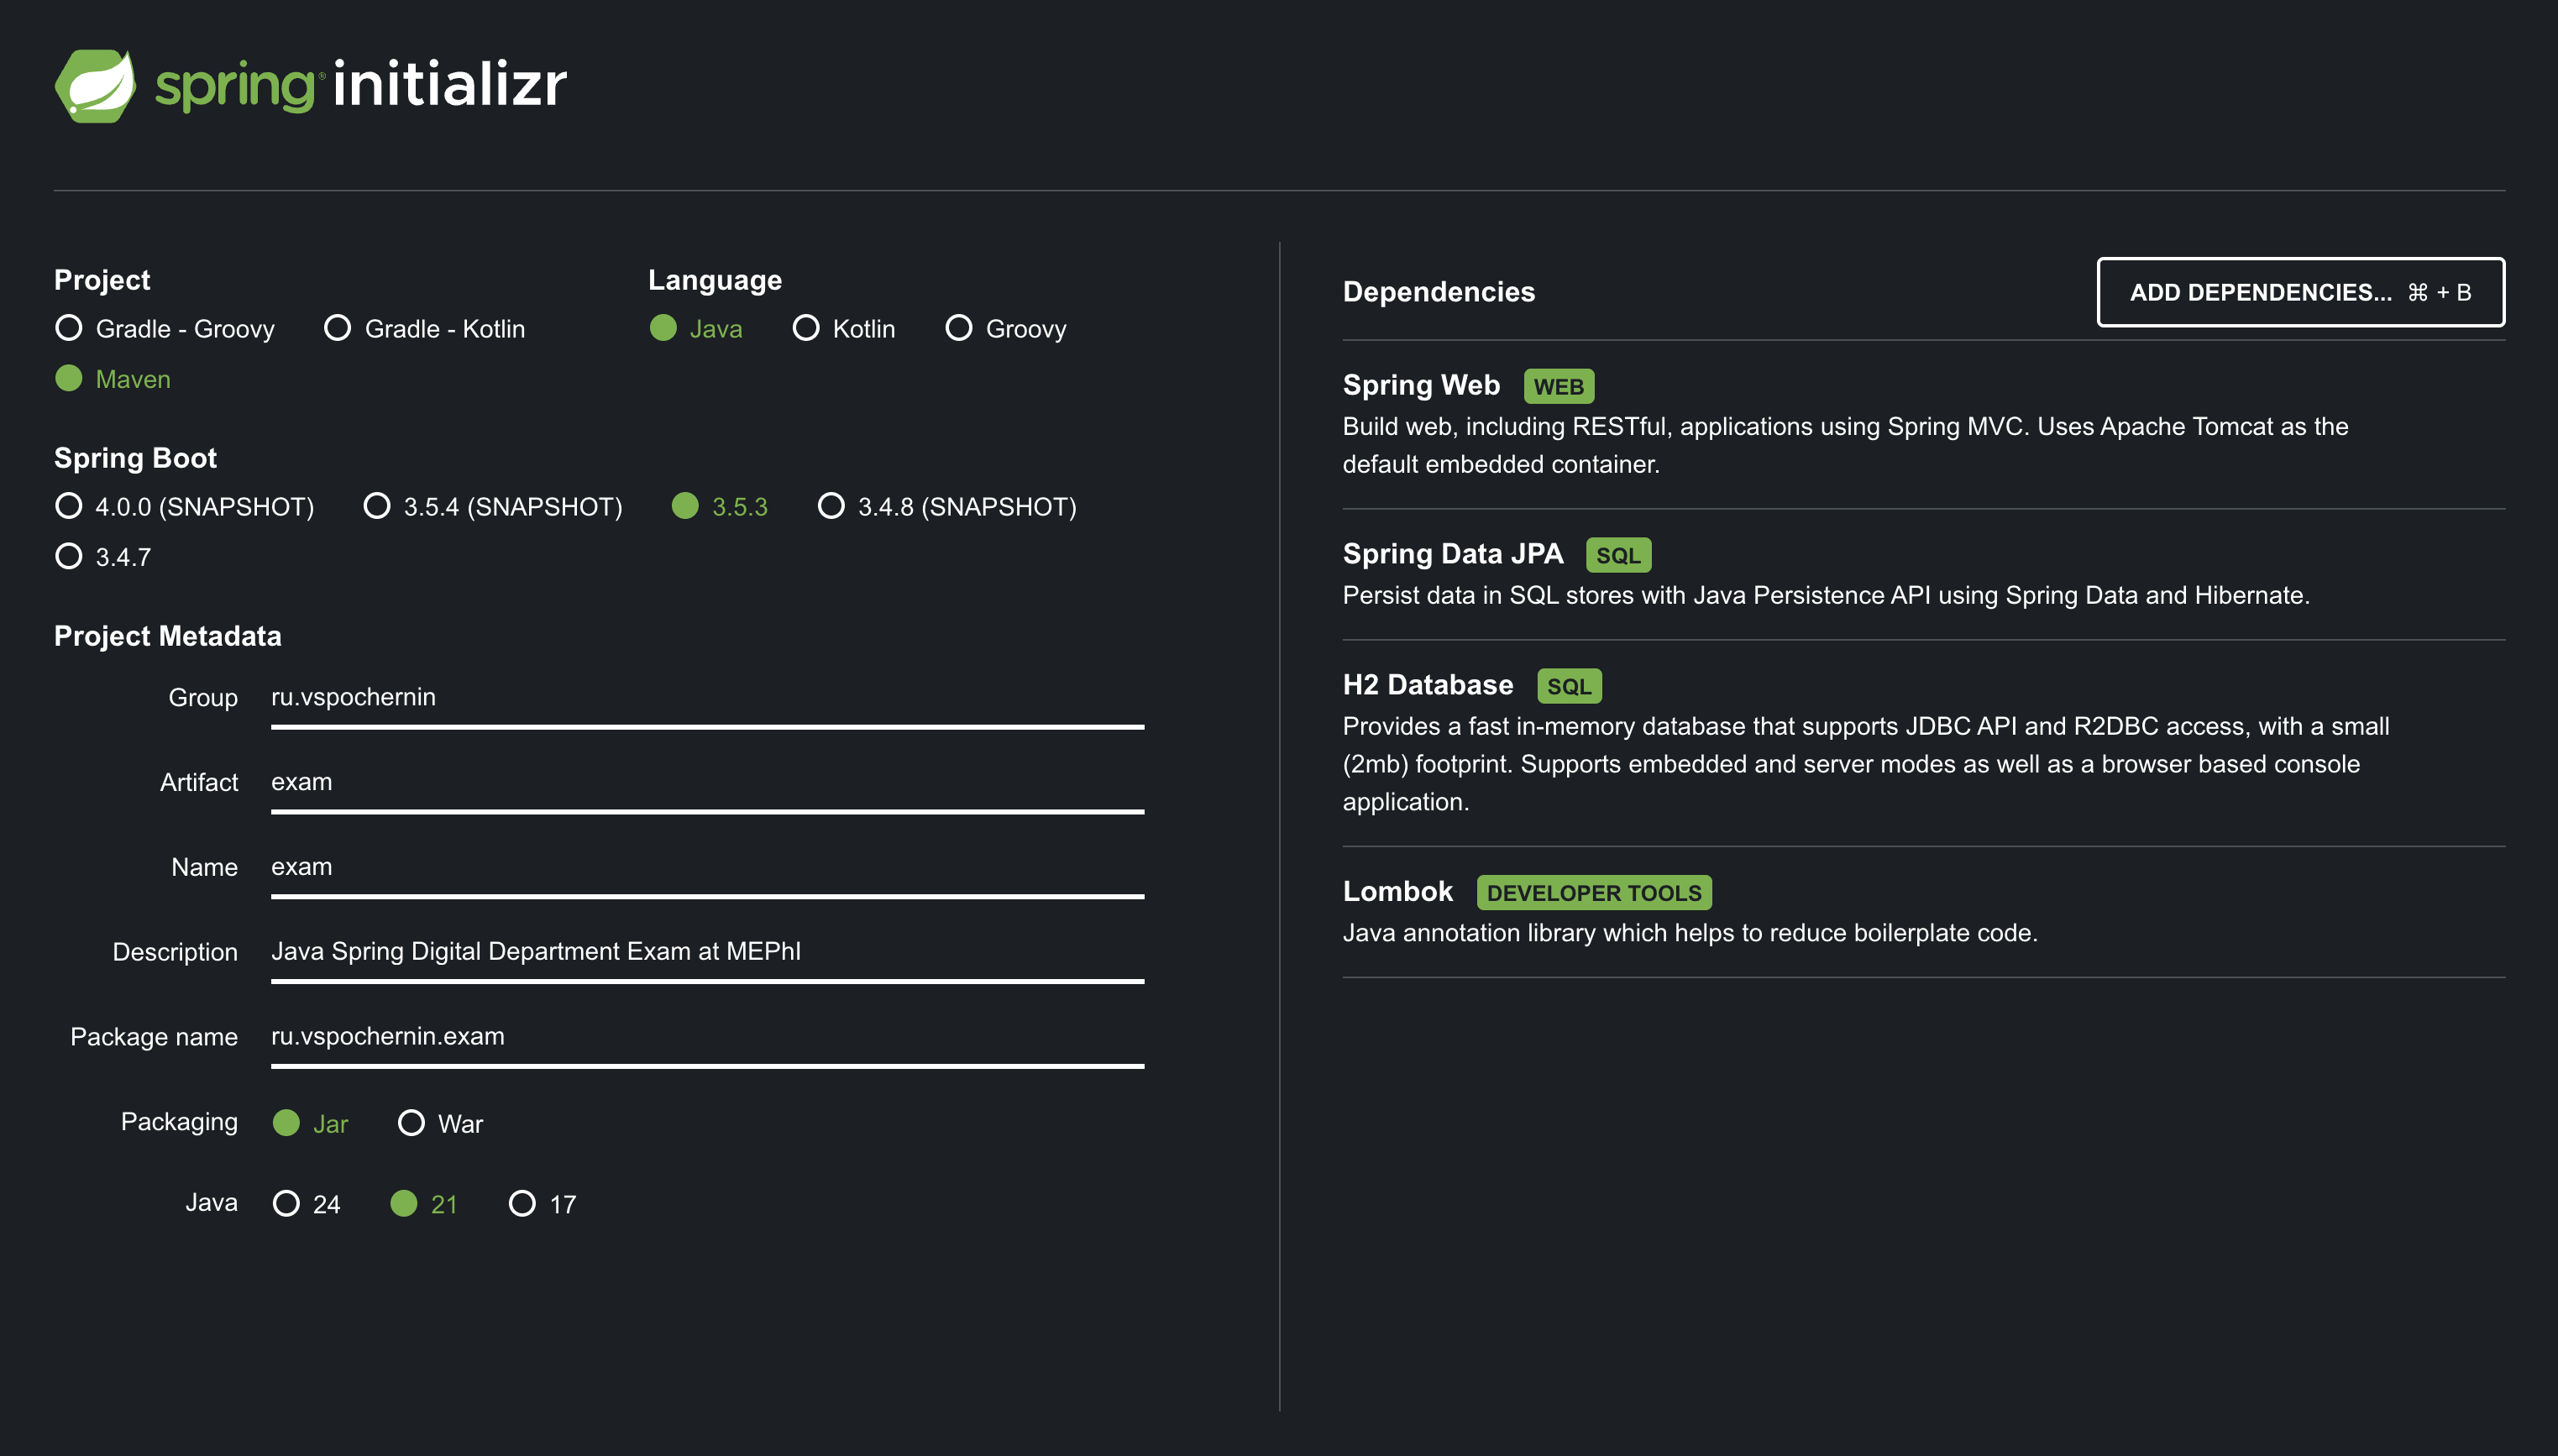
\includegraphics[width=17cm]{resources/1.png}
	\caption{Инициализация проекта}
\end{figure}

Мы будем использовать Java версии 21, сборщик Maven, а также актуальную на момент написания отчета версию Spring Boot - 3.5.3.


Из зависимостей были выбраны:

\begin{itemize}
	\item Spring Web - для создания сервера, который сможет отвечать на HTTP запросы.
	\item Spring Data JPA - для взаимодействия с нашей H2 базой данных с помощью объектно-реляционного отображения.
	\item H2 Database - драйвер для работы H2 базы данных.
	\item Lombok - вспомогательный инструмент для уменьшения количества boilerplate кода.
\end{itemize}

\subsection{Разработка}

\subsubsection{Пакет model}

Для начала реализуем классы-модели.

Создадим enum \texttt{Country}, задающий 5 стран:

\normalsize
\inputminted[frame=single]{Java}{../src/main/java/ru/vspochernin/exam/model/Country.java}
\large

А также класс пользователя, который будет связан с таблицей \texttt{users} базы данных:

\normalsize
\inputminted[frame=single]{Java}{../src/main/java/ru/vspochernin/exam/model/User.java}
\large

Важными моментами здесь является аннотация \texttt{@Table(name = "users")}, задающая название таблицы БД, а также аннотация \texttt{@Enumerated(EnumType.STRING)}, объясняющая, что enum нужно обрабатывать как строку (без нее в базу записывались бы порядковые номера). \texttt{@GeneratedValue(strategy = GenerationType.IDENTITY)} над полем \texttt{id} делегирует установку ID на уровень базы данных, нам не нужно будет задумываться об этом.

\subsubsection{Пакет repository}

Далее реализуем класс-репозиторий для пользователя:

\normalsize
\inputminted[frame=single]{Java}{../src/main/java/ru/vspochernin/exam/repository/UserRepository.java}
\large

Здесь мы добавили метод \texttt{findByAgeGreaterThanEqualOrderByFirstNameAsc} для того, чтобы использовать его в эндпоинте \texttt{additional-info}.

% \it{Раздел должен содержать описание функционала реализованного приложения. Описание может сопровождаться скриншотами, которые должны содержать информацию об успешном выполнении каждого запроса (в т.ч.: входящий запрос, тело запроса, статус и результат выполнения запроса).}

\newpage
\section{Заключение}

% \it{Раздел должен содержать общие выволды по работе}.

\iffalse
\section{Описание проекта}

Система управления личными финансами представляет собой приложение, предоставляющее возможность пользователям добавлять доходы и расходы, просматривать статистику по финансам, а также устанавливать бюджеты и категории.

Приложение написано в строгом соответствии с критериями, описанными в

\texttt{README.md} (соответствие критериям будет показано ниже).

\subsection{Используемые технологии}

\begin{itemize}
	\item \texttt{Java} - язык программирования.
	\item \texttt{Spring} - основной фреймворк.
	\item \texttt{PostgreSQL} - используемая СУБД.
	\item \texttt{Maven} - система сборки проекта.
	\item \texttt{Flyway} - инструмент для применения файлов миграций БД.
	\item \texttt{Lombok} - библиотека для сокращения шаблонного кода.
	\item \texttt{Bcrypt} - инструмент для хеширования паролей.
\end{itemize}

\subsection{Описание модулей}

Вкратце рассмотрим кодовую базу проекта:.

\begin{itemize}
	\item Пакет \texttt{command}: содержит в себе классы, отвечающие за работу интерфейса командной строки, такие как сама команда, типы команд, а также сам класс интерфейса.
	\item Пакет \texttt{context}: содержит класс, отвечающий за переменные контекста приложения.
	\item Пакет \texttt{entity}: содержит классы моделей данных (связанных с базой при помощи \texttt{ORM}).
	\item Пакет \texttt{exception}: содержит в себе класс-исключение, связанное с системой управления личными финансами.
	\item Пакет \texttt{handler}: содержит в себе классы, реализующие паттерн \texttt{Стратегия} и используемые для обработки команд.
	\item Пакет \texttt{repository}: содержит в себе классы - \texttt{JPA} репозитории.
	\item Пакет \texttt{utils}: содержит в себе различные утильные классы.
	\item Папка \texttt{migration}: содержит в себе файлы миграции БД, которые устанавливают схему и наполняют базу тестовыми данными.
\end{itemize}

\subsection{Схема БД}

База данных проекта имеет следующую схему:

\begin{figure}[H]
	\centering
	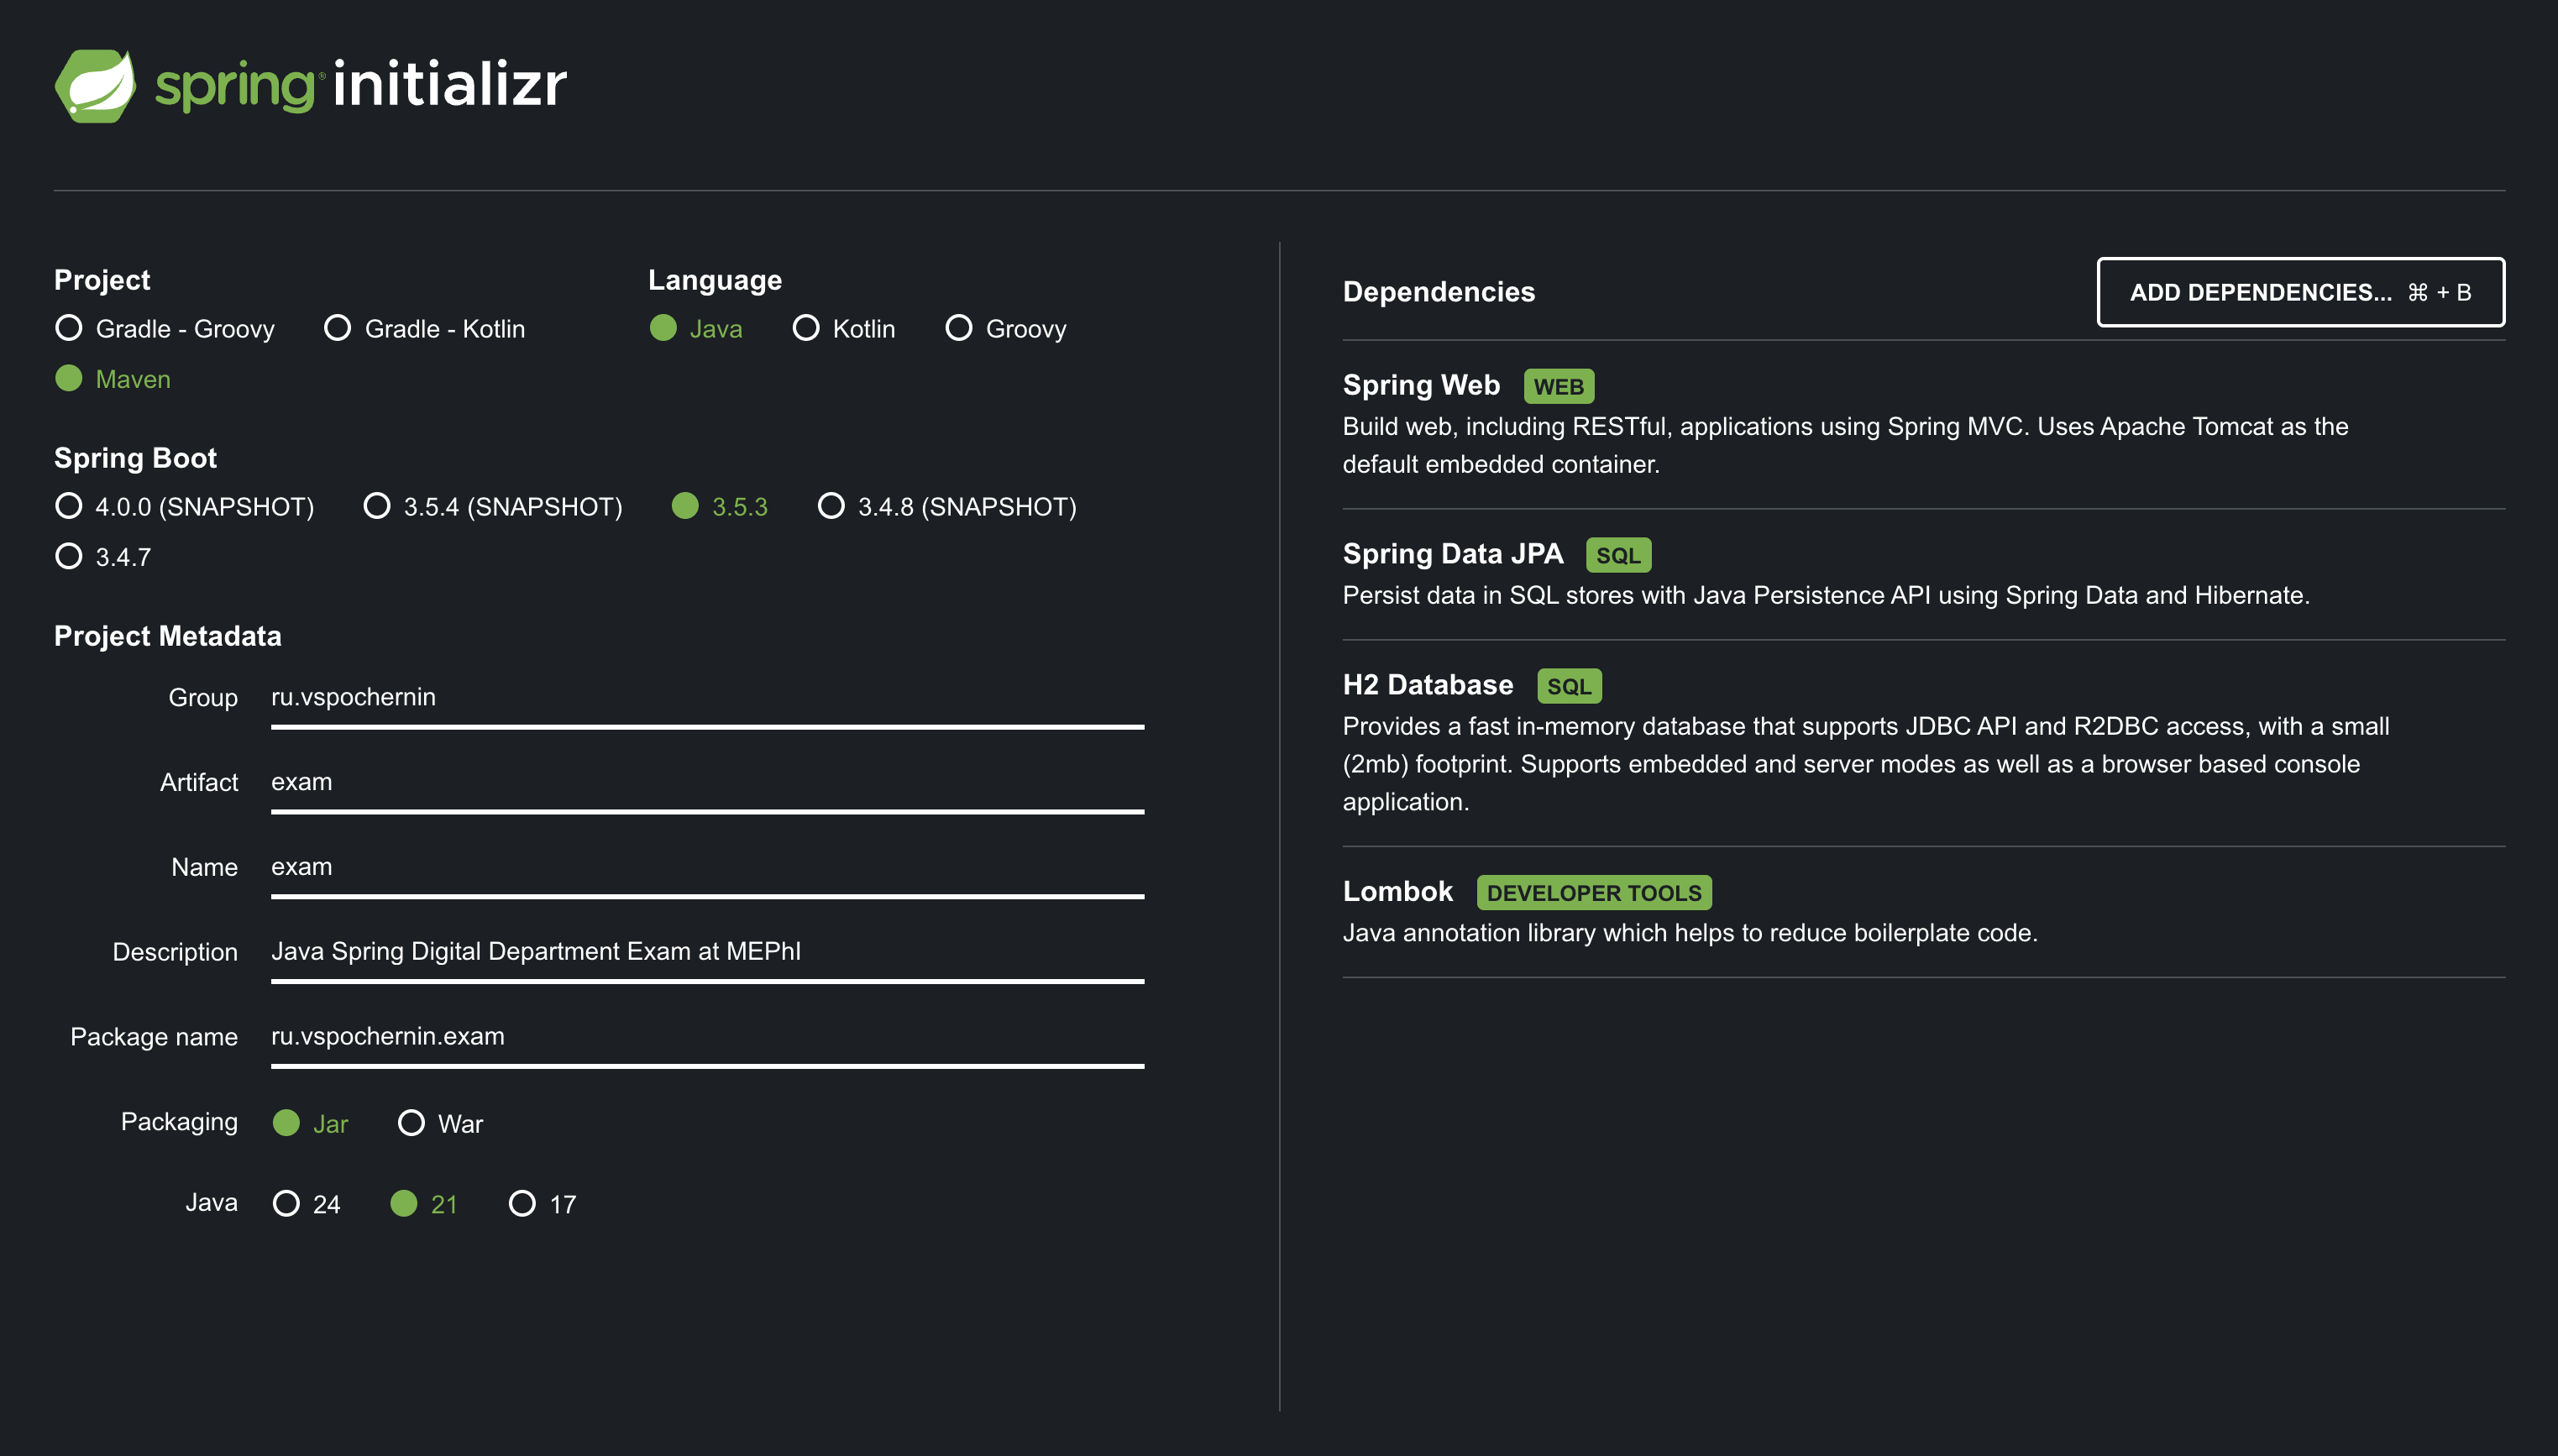
\includegraphics[width=17cm]{resources/1.png}
	\caption{Схема БД}
\end{figure}

\begin{itemize}
	\item Таблица \texttt{users} содержит информацию о пользователях.
	\begin{itemize}
		\item \texttt{id} выступает ключом записи.
		\item \texttt{login} - логин, присутствует требование уникальности.
		\item \texttt{password} - пароль, будет храниться в зашифрованном виде.
	\end{itemize}
	\item Таблица \texttt{categories} содержит информацию о категориях пользователей.
	\begin{itemize}
		\item \texttt{id} выступает ключом записи.
		\item \texttt{user\_id} - ссылка на таблицу \texttt{users}, у каждого пользователя свои категории.
		\item \texttt{title} - название категории.
		\item \texttt{type} - тип категории, возможные значения \texttt{INCOME} (доход) или \texttt{EXPENSE} (расходы).
		\item \texttt{budget} - бюджет на категорию в копейках, может отсутствовать.
		\item Присутствует требование уникальности по паре (\texttt{user\_id}, \texttt{title}).
	\end{itemize}
	\item Таблица \texttt{transactions} содержит информацию о конкретных транзакциях (доходах, расходах).
	\begin{itemize}
		\item \texttt{id} выступает ключом записи.
		\item \texttt{category\_id} - ссылка на таблицу \texttt{categories}. Каждая транзакция связана с какой-либо категорией.
		\item \texttt{amount} - сумма транзакции в копейках.
		\item \texttt{datetime} - метка времени совершения транзакции (по умолчанию выставляется \texttt{current\_timestamp}).
	\end{itemize}
\end{itemize}

\newpage
\section{Инструкции по запуску кода}

Для того, чтобы запустить код, необходимо иметь

\begin{itemize}
	\item \texttt{Java 17} (полагаю, что версии выше также подойдут).
	\item \texttt{Docker} (необходим для быстрого поднятия БД, но можно поднимать руками).
	\item \texttt{Maven} (поддерживается в \texttt{IntelliJ IDEA}).
\end{itemize}

Запустим наш проект. Для начала, перейдем в директорию, содержащую конфигурационный файл докера - \texttt{/src/main/resources/db}, затем запустим базу данных в \texttt{detach} режиме командой \texttt{docker compose up -d}

\begin{figure}[H]
	\centering
	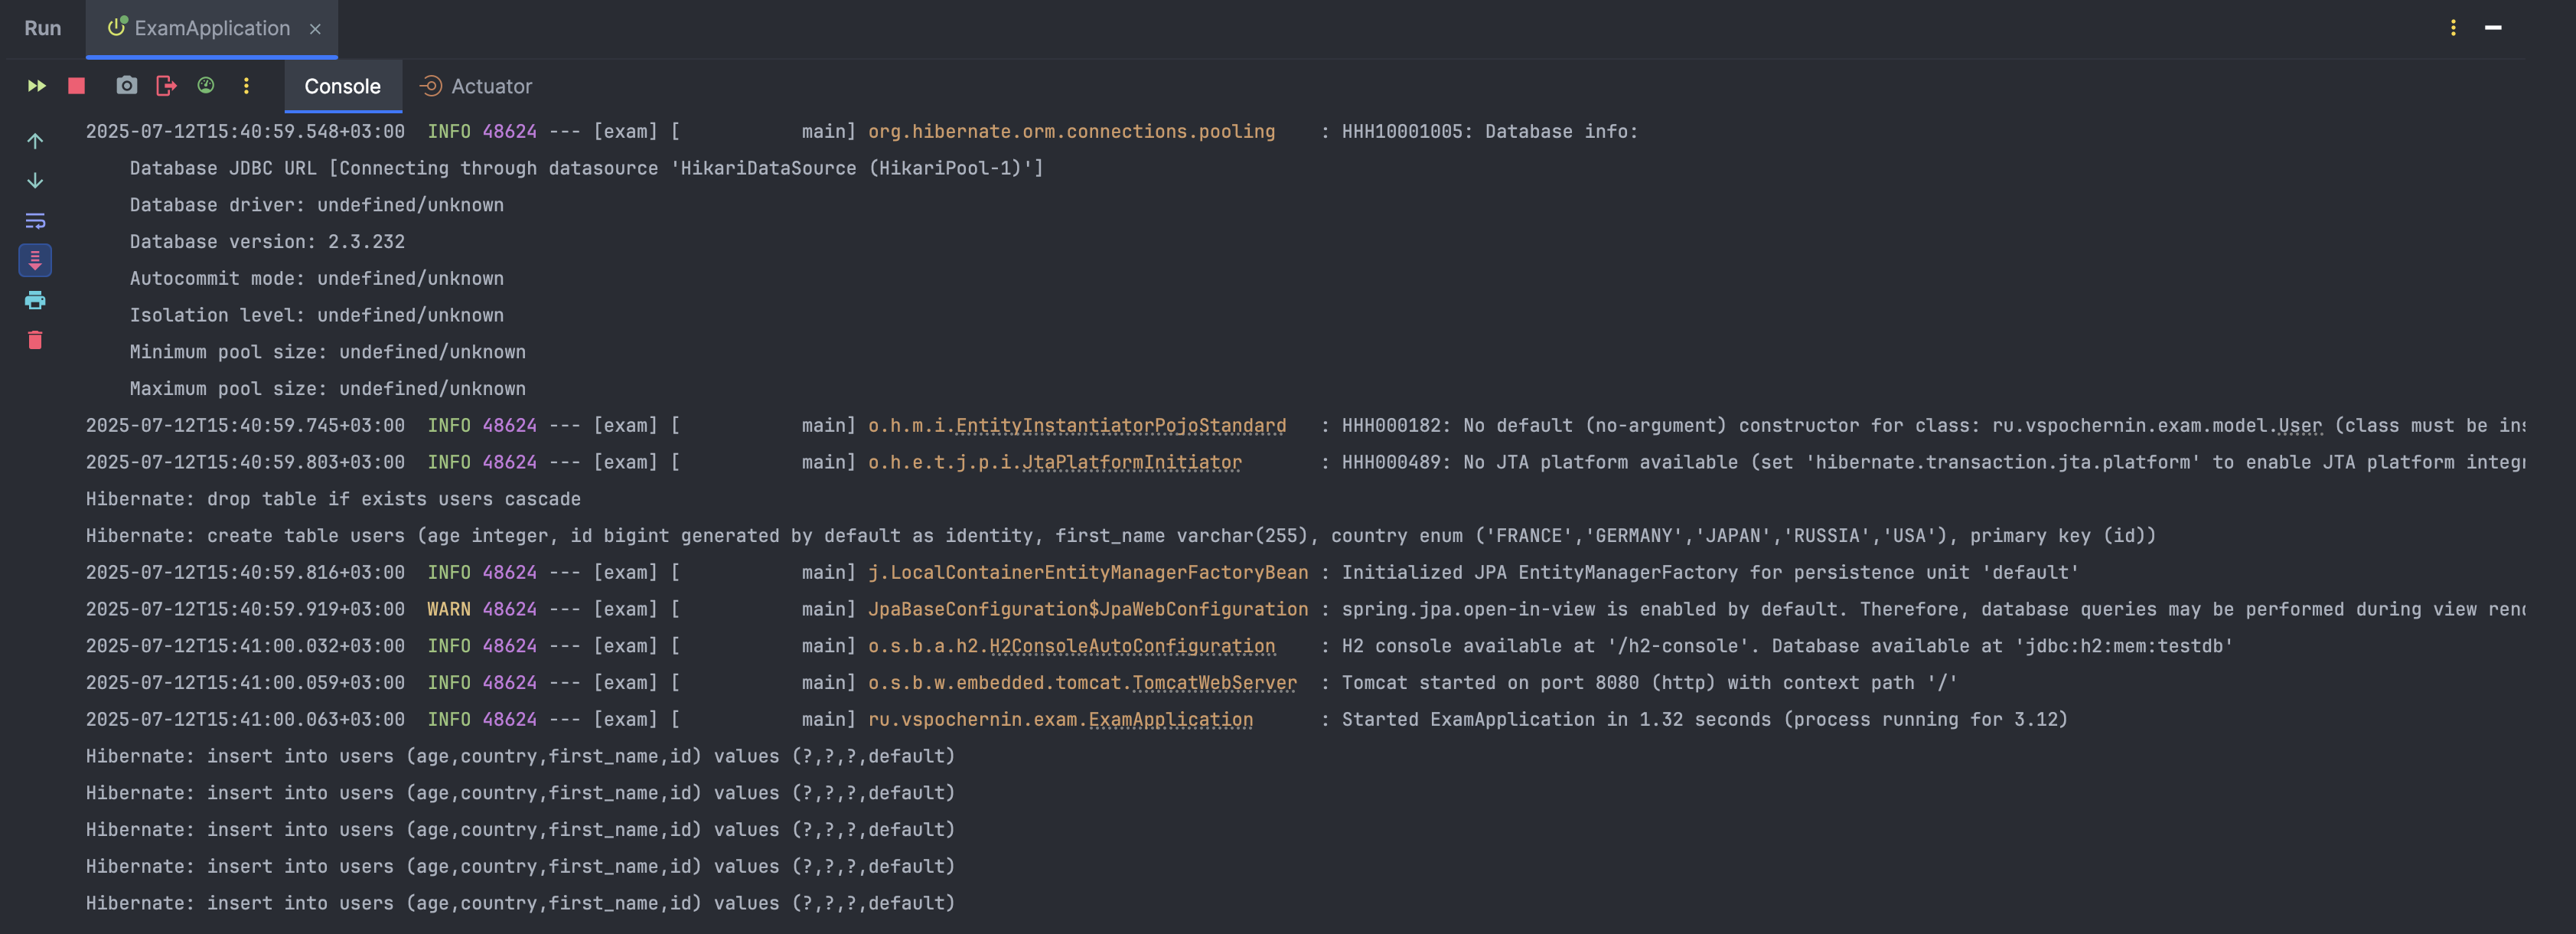
\includegraphics[width=17cm]{resources/2.png}
	\caption{Запуск БД}
\end{figure}

Чтобы запустить проеект, необходимо запустить \texttt{main()} метод из класса

\texttt{FinanceManagementApplication} с помощью \texttt{IntelliJ IDEA} (идея при запуске проекта должна автоматически скачать все зависимости).

После запуска кода мы увидим приветственное сообщение с описанием всех команд, а также требованиями к некоторым аргументам.

PS. Вероятно, это относится только к моему компьютеру, но я получал ошибку при запуске, пока не добавил в конфигурацию запуска в VM Options

\texttt{-Djava.rmi.server.hostname=localhost}

\begin{figure}[H]
	\centering
	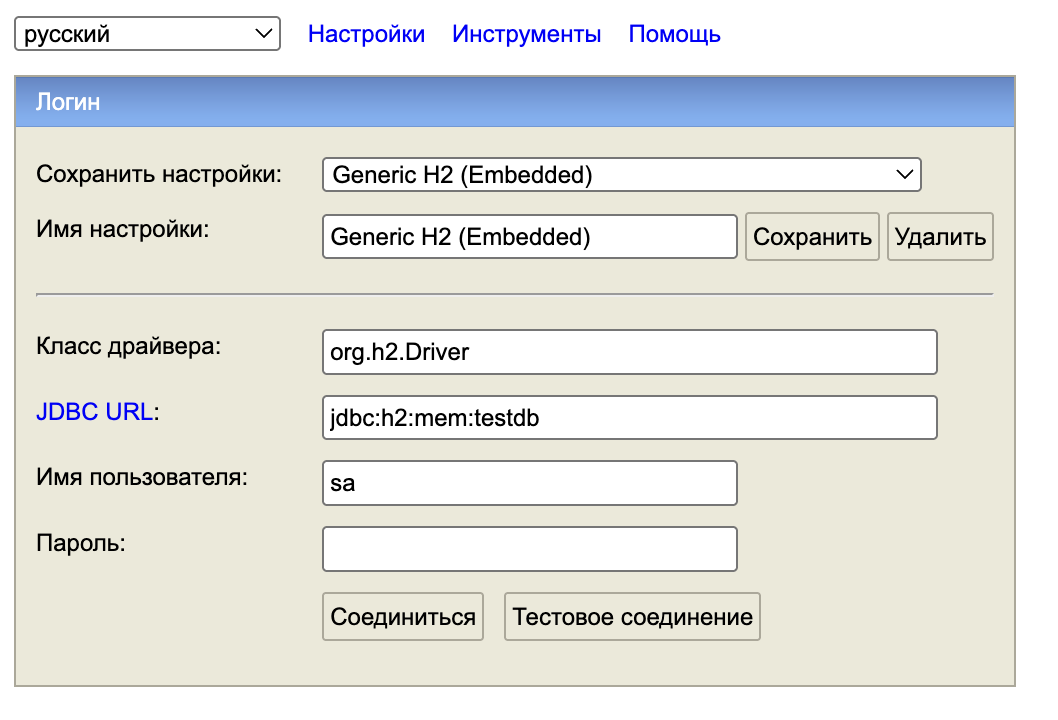
\includegraphics[width=17cm]{resources/3.png}
	\caption{Запуск кода}
\end{figure}

\newpage
\section{Демонстрация работы}

Проведем демонстрацию работы всех команд приложения.

\subsection{Вывод сообщения помощи (help)}

Команда \texttt{help} выводит сообщение с описанием всех команд, а также с требованиями к некоторым аргументам.

\begin{figure}[H]
	\centering
	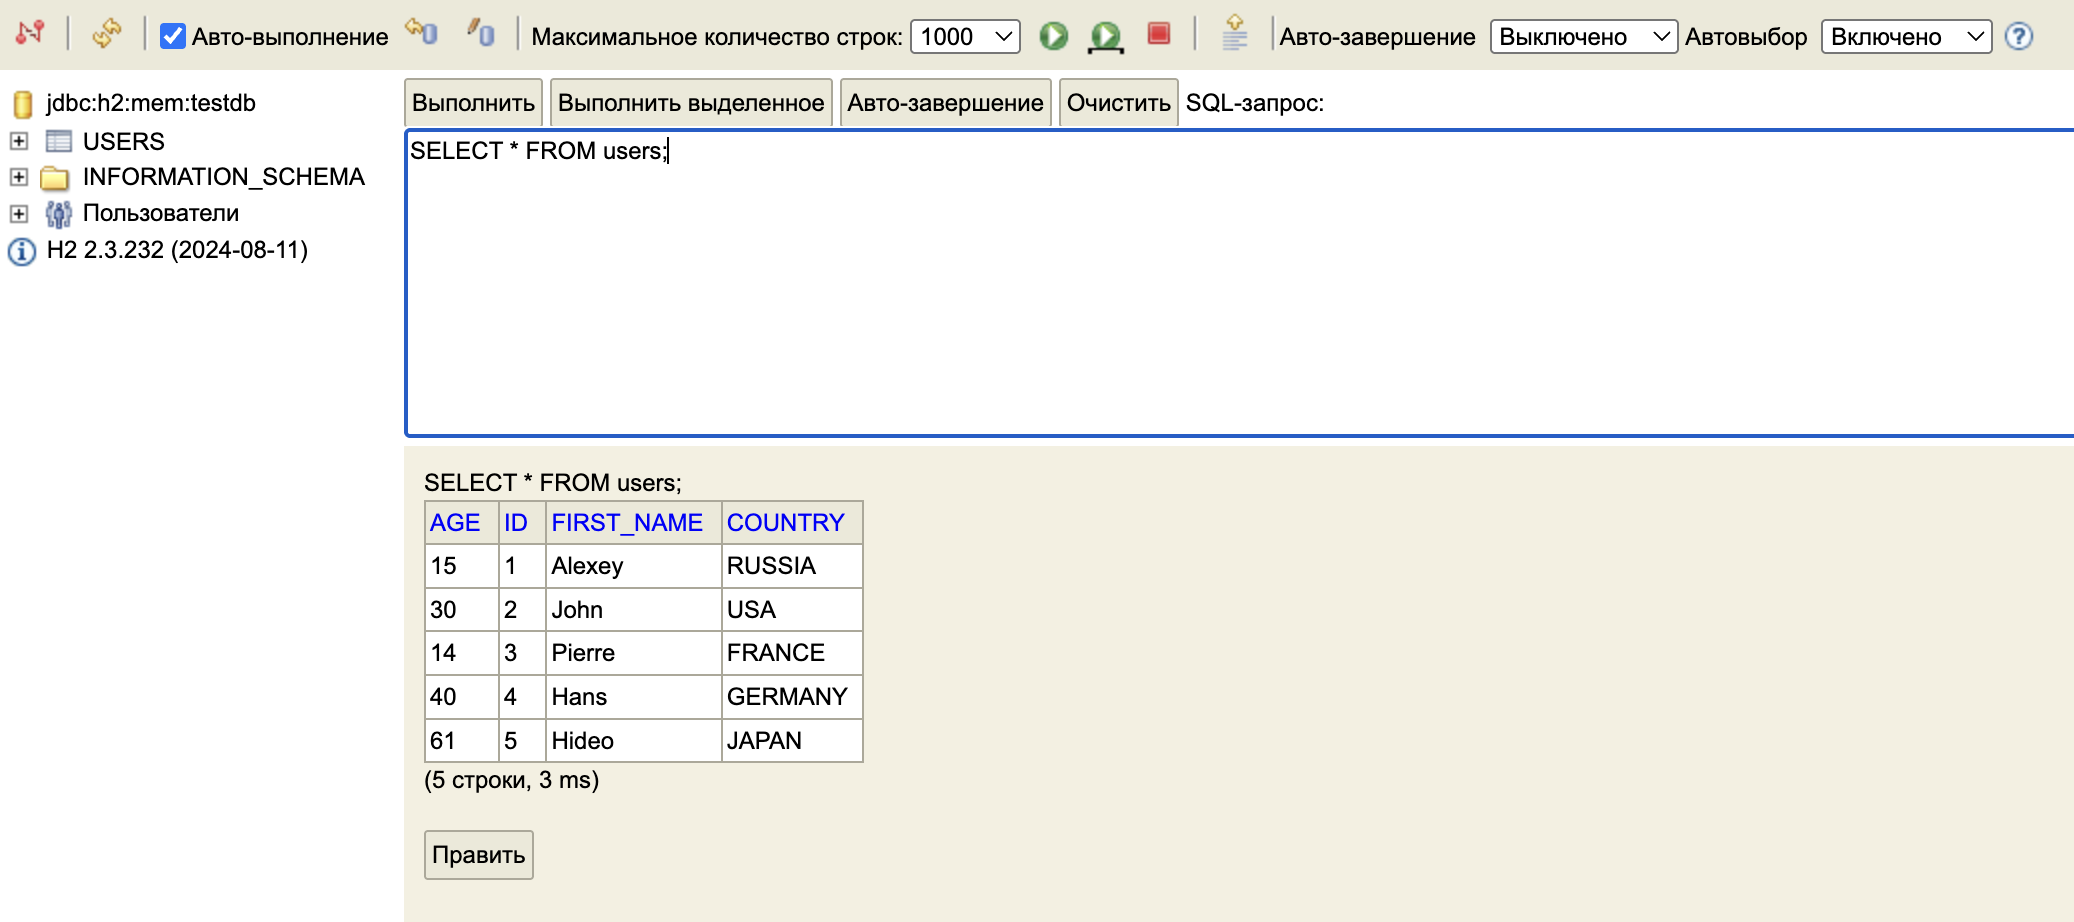
\includegraphics[width=17cm]{resources/4.png}
	\caption{Вывод сообщения помощи}
\end{figure}

\subsection{Регистрация (register)}

Команда \texttt{register} регистрирует нового пользователя в системе. Пароль при этом хэшируется алгоритмом \texttt{Bcrypt}.

\begin{figure}[H]
	\centering
	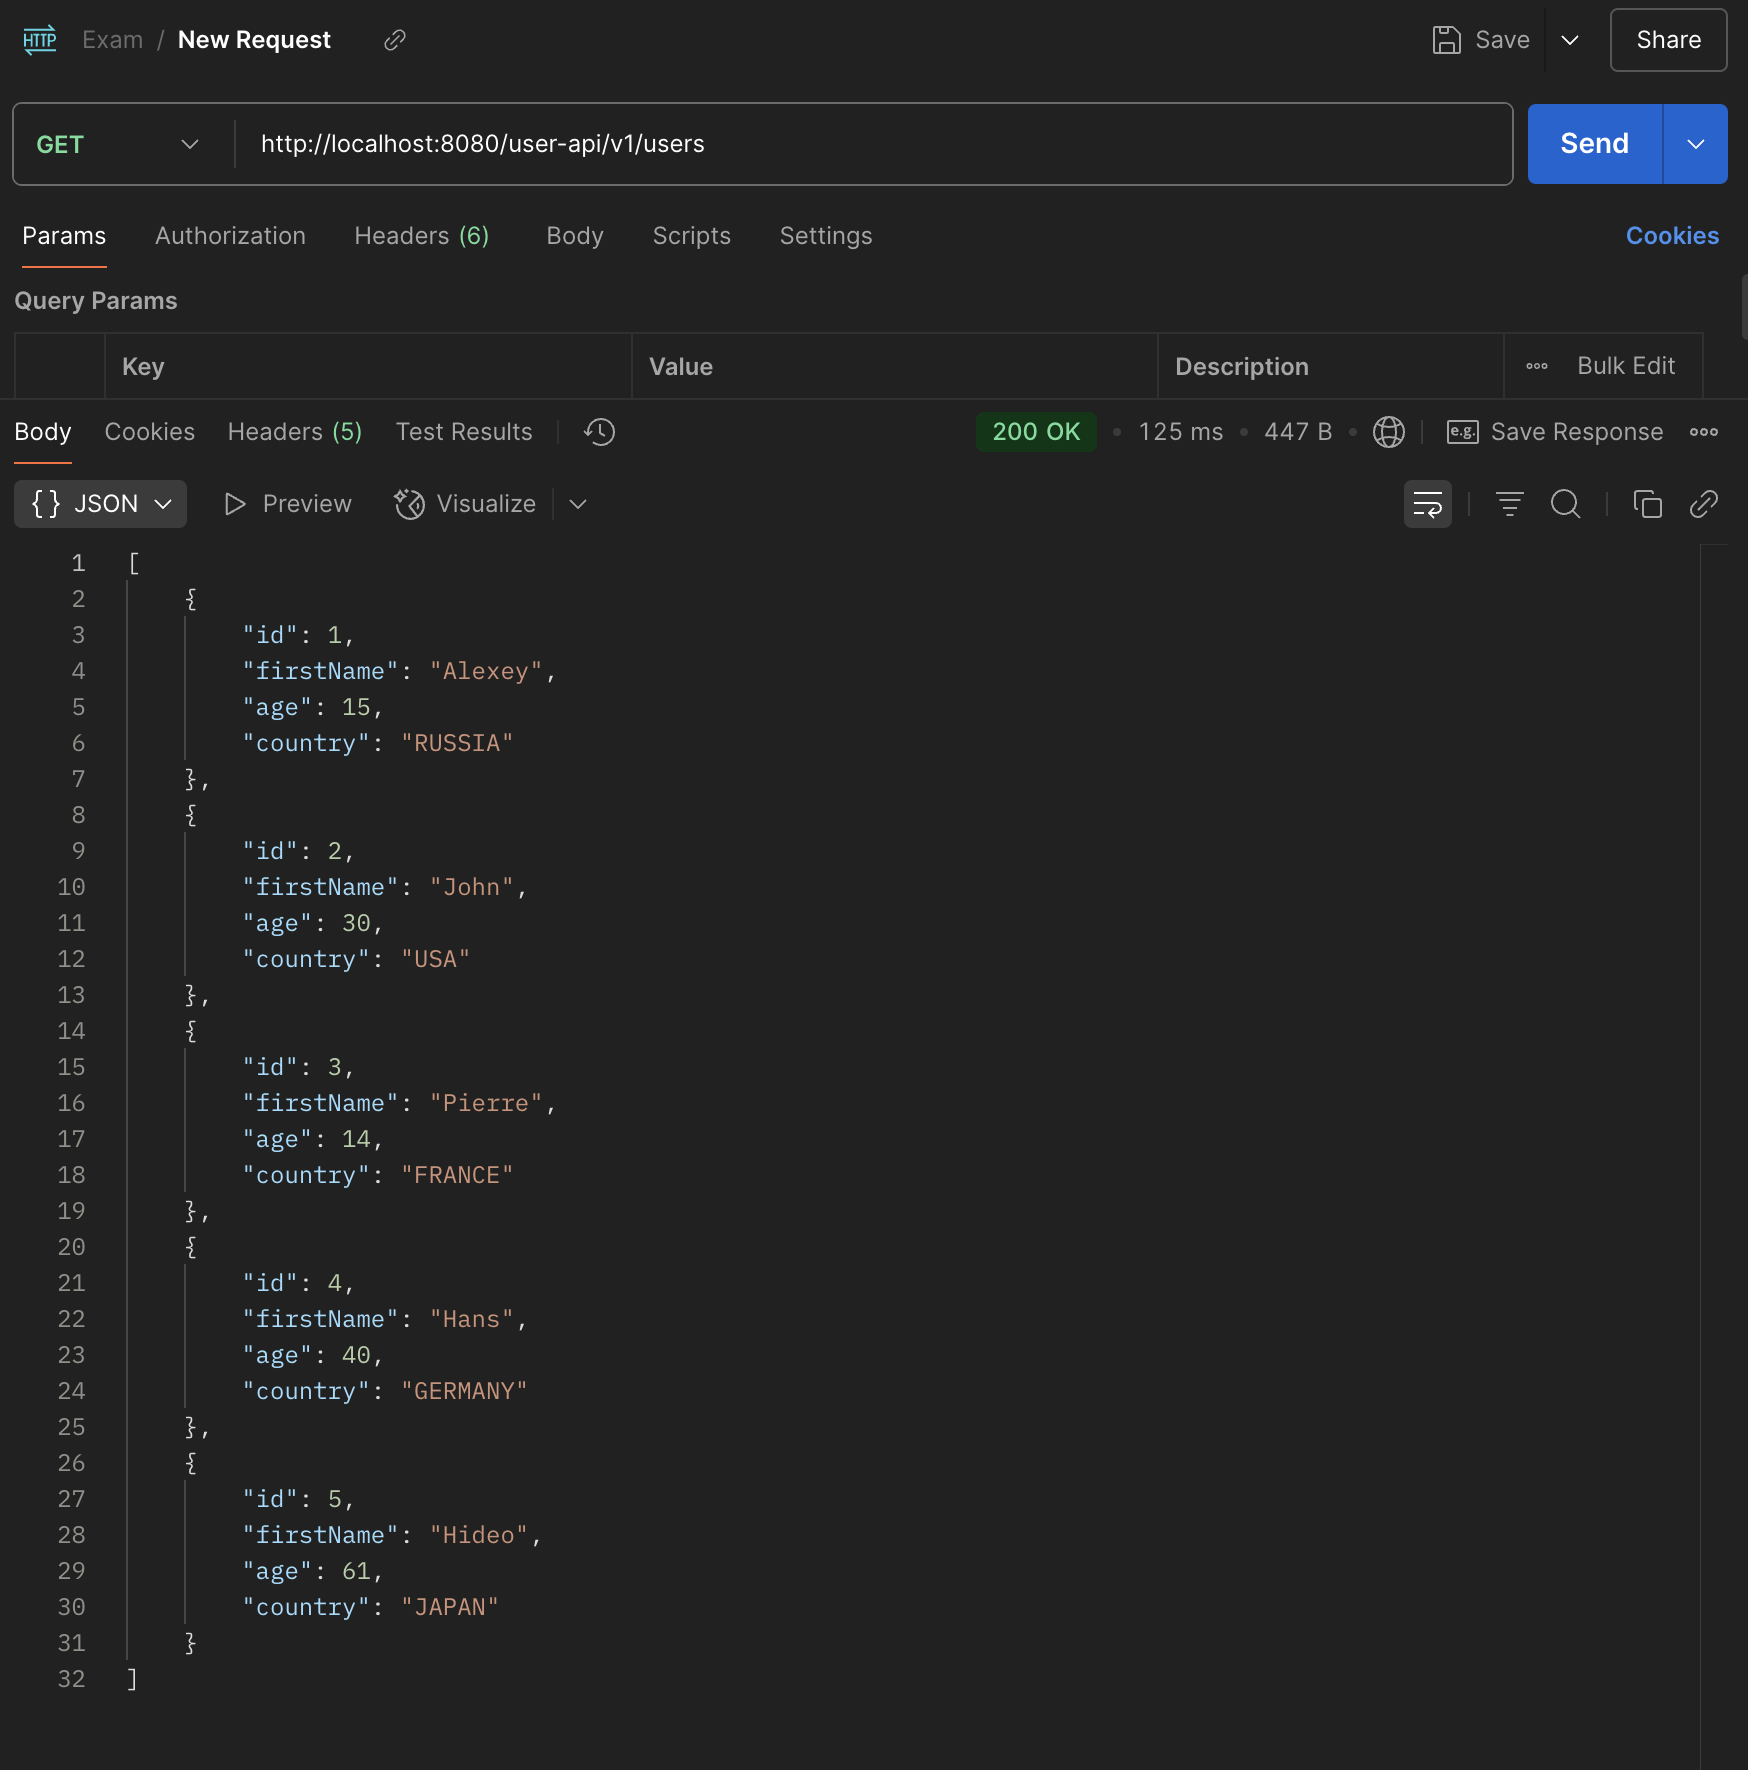
\includegraphics[width=13cm]{resources/5.png}
	\caption{Проведение регистрации}
\end{figure}

\subsection{Аутентификация (login)}

Команда \texttt{login} проводит аутентификацию пользователя. При этом сравниваются хеши переданного и сохраненного в базе паролей.

\begin{figure}[H]
	\centering
	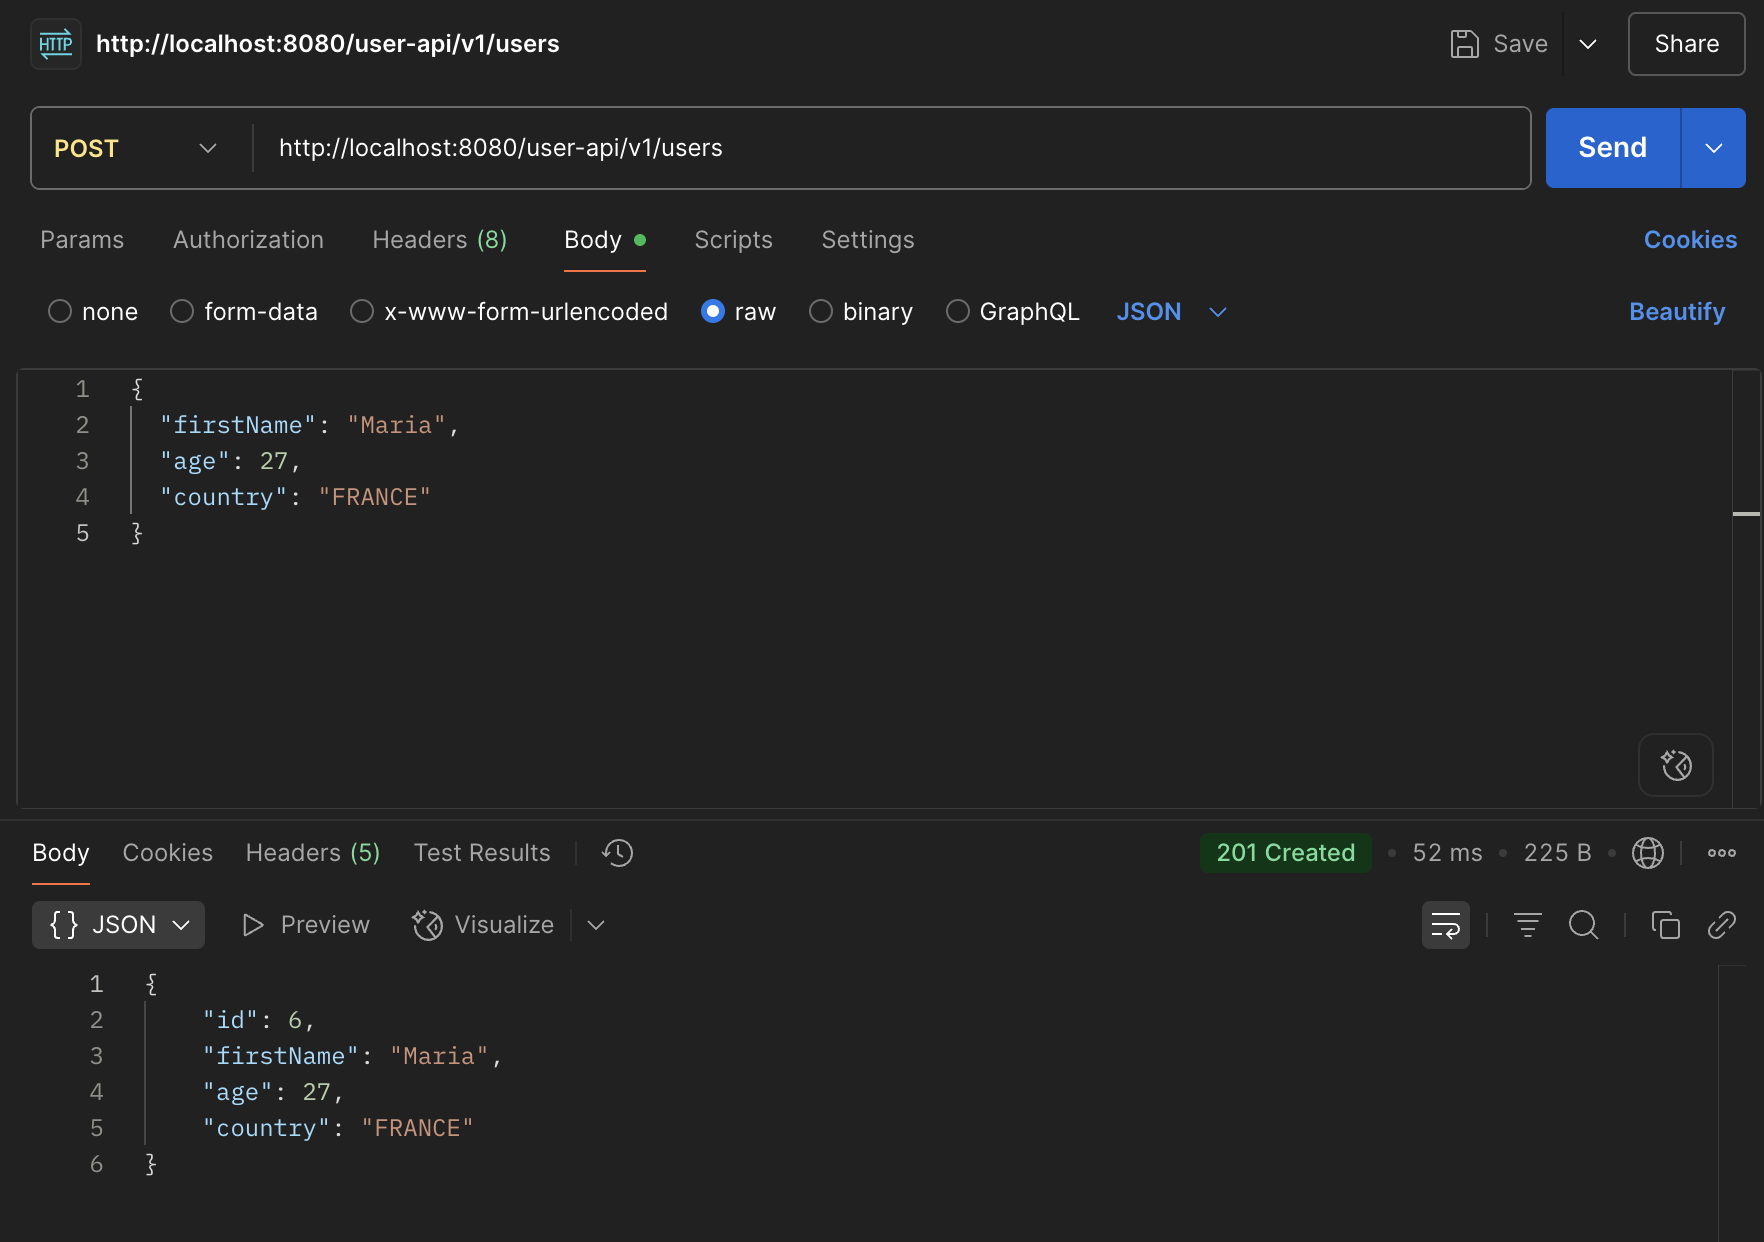
\includegraphics[width=13cm]{resources/6.png}
	\caption{Проведение аутентификации}
\end{figure}

\subsection{Создание категории (category)}

Команда \texttt{category} создает категорию дохода или расхода. Создадим категории согласно примеру из \texttt{README.md}:

\begin{figure}[H]
	\centering
	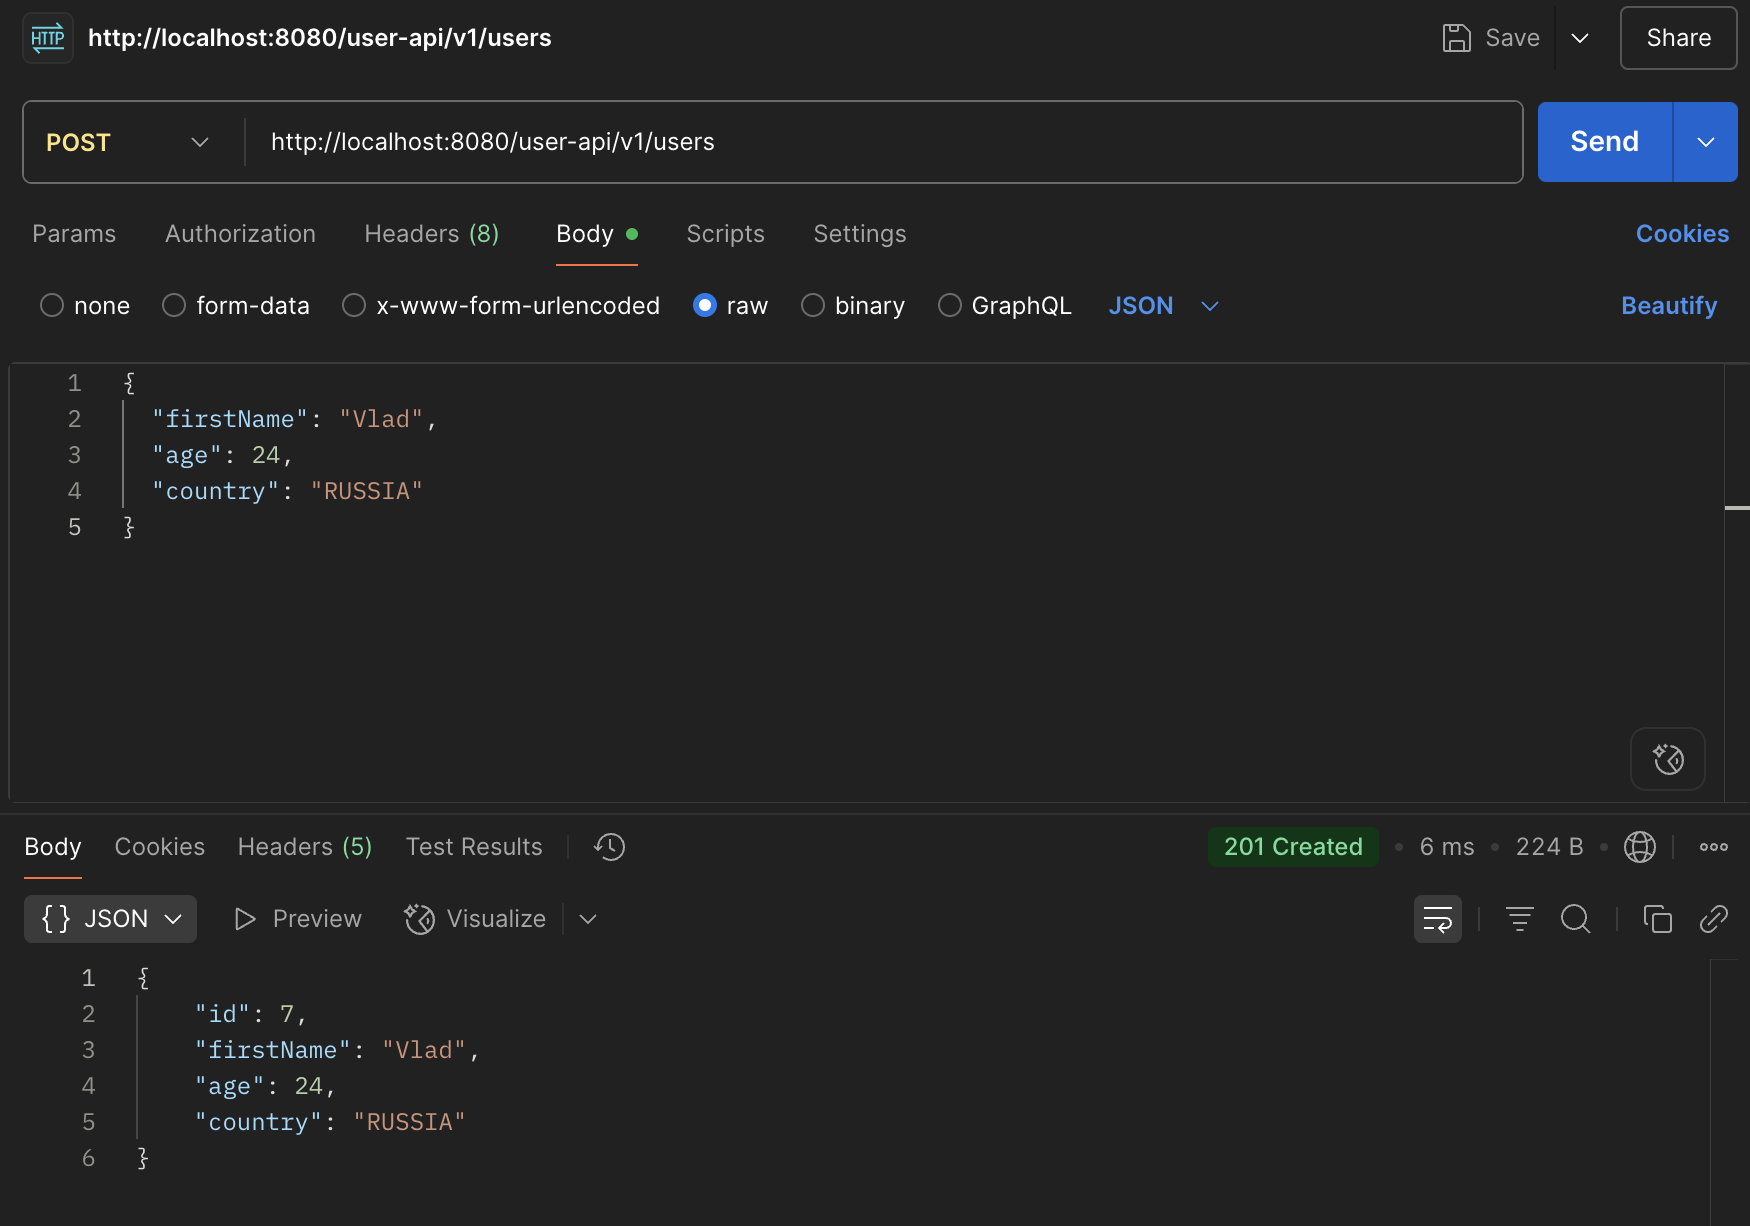
\includegraphics[width=10cm]{resources/7.png}
	\caption{Создание категорий}
\end{figure}

\subsection{Установка бюджета (budget)}

Команда \texttt{budget} устанавливает бюджет на определенную категорию расхода. Установим бюджеты согласно примеру из \texttt{README.md}.

\begin{figure}[H]
	\centering
	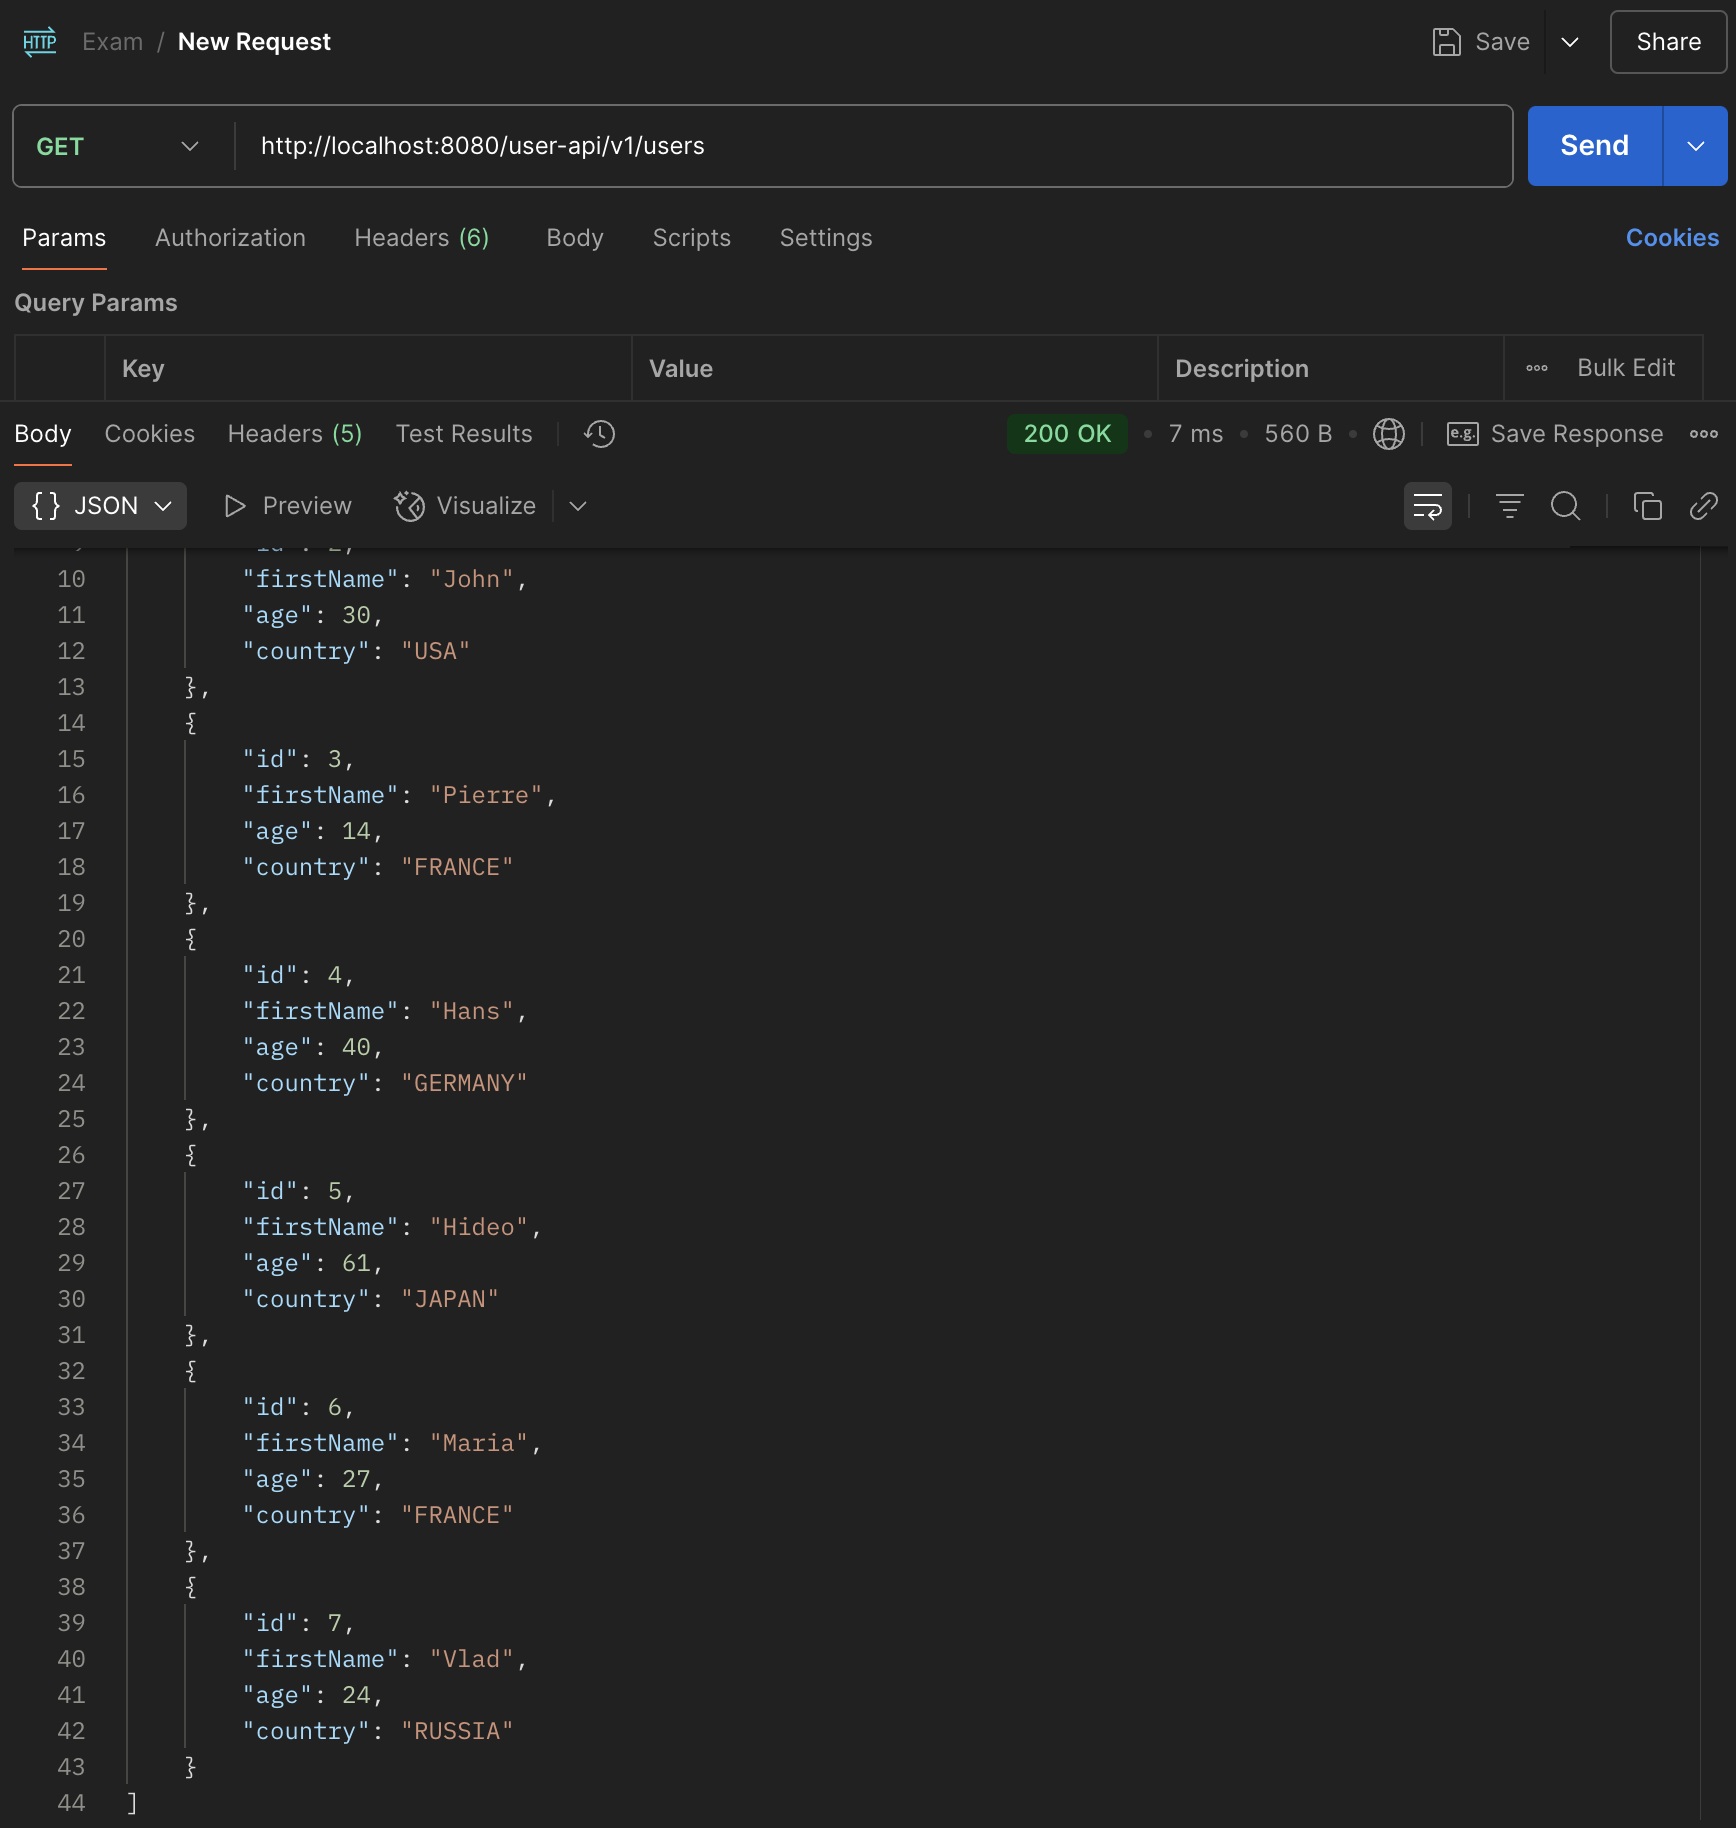
\includegraphics[width=10cm]{resources/8.png}
	\caption{Установка бюджетов}
\end{figure}

\subsection{Добавление транзакции (transaction)}

Команда \texttt{transaction} добавляет транзакцию по одной из категории дохода или расхода. Добавим транзакции согласно примеру из \texttt{README.md}.

Также здесь можно будет заметить уведомления о превышении расходов над доходами, а также о превышении конкретного установленного бюджета.

\begin{figure}[H]
	\centering
	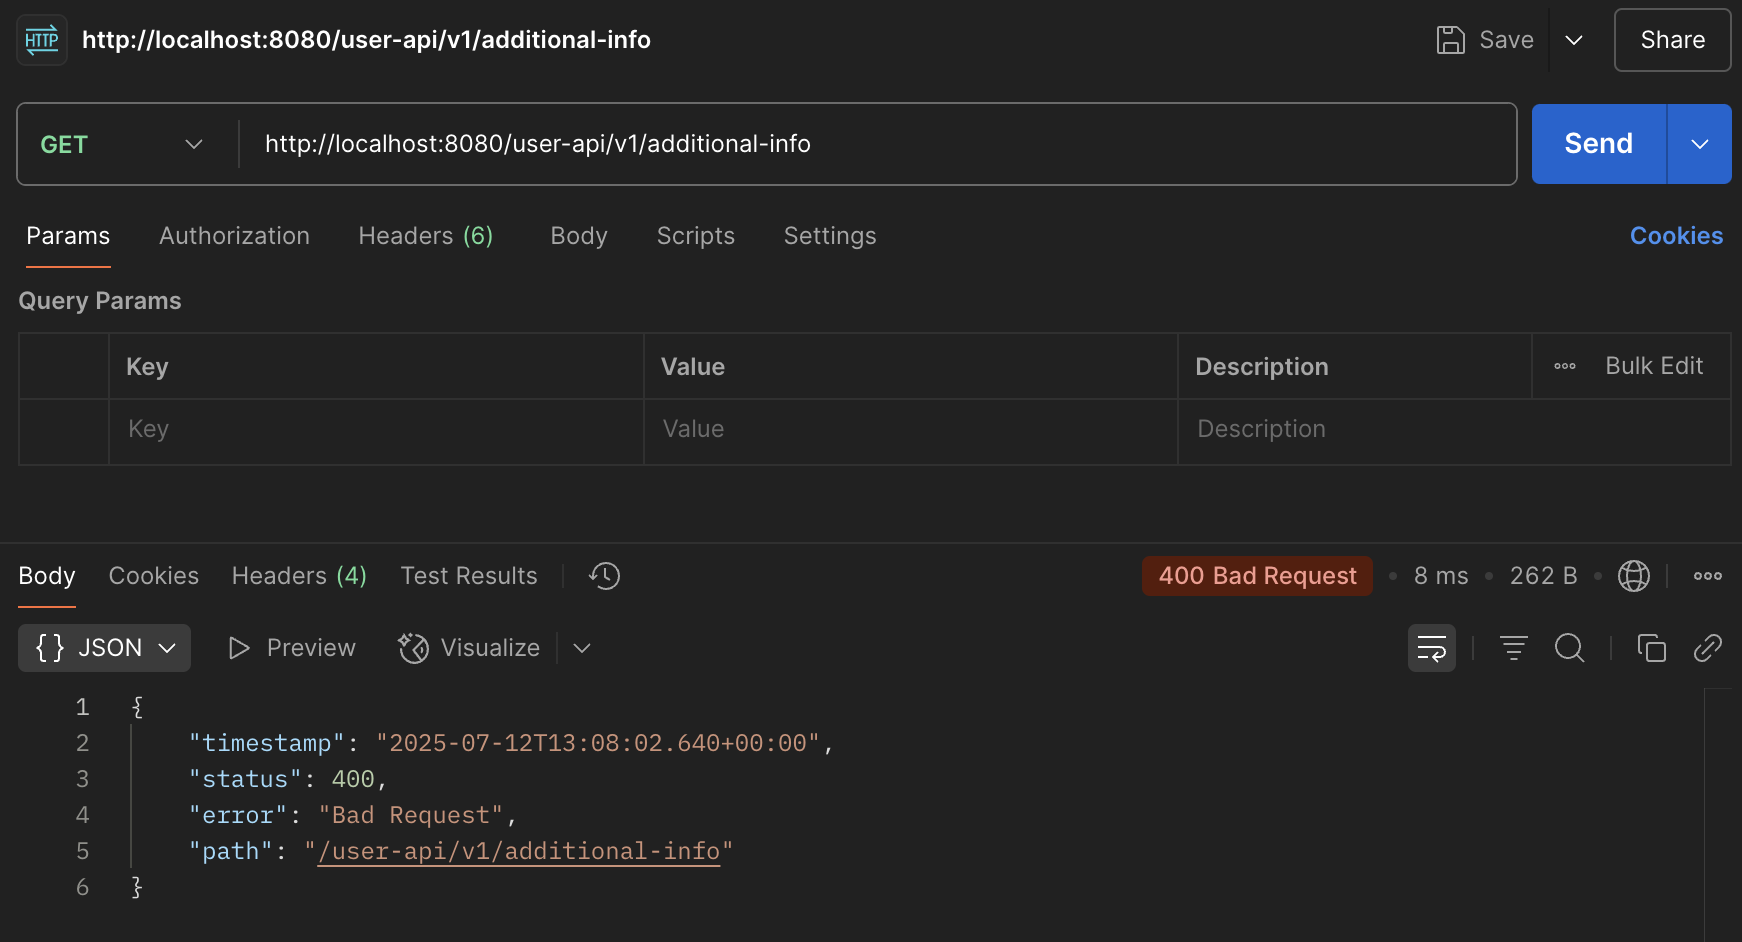
\includegraphics[width=13cm]{resources/9.png}
	\caption{Добавление транзакций}
\end{figure}

\subsection{Вывод подробной информации по доходам/расходам/бюджетам (info)}

Команда \texttt{info} выводит подробную информацию по доходам/расходам/бюджетам пользователя. Убедимся, что ее вывод будет таким же, какой ожидается в \texttt{README.md}:

\begin{figure}[H]
	\centering
	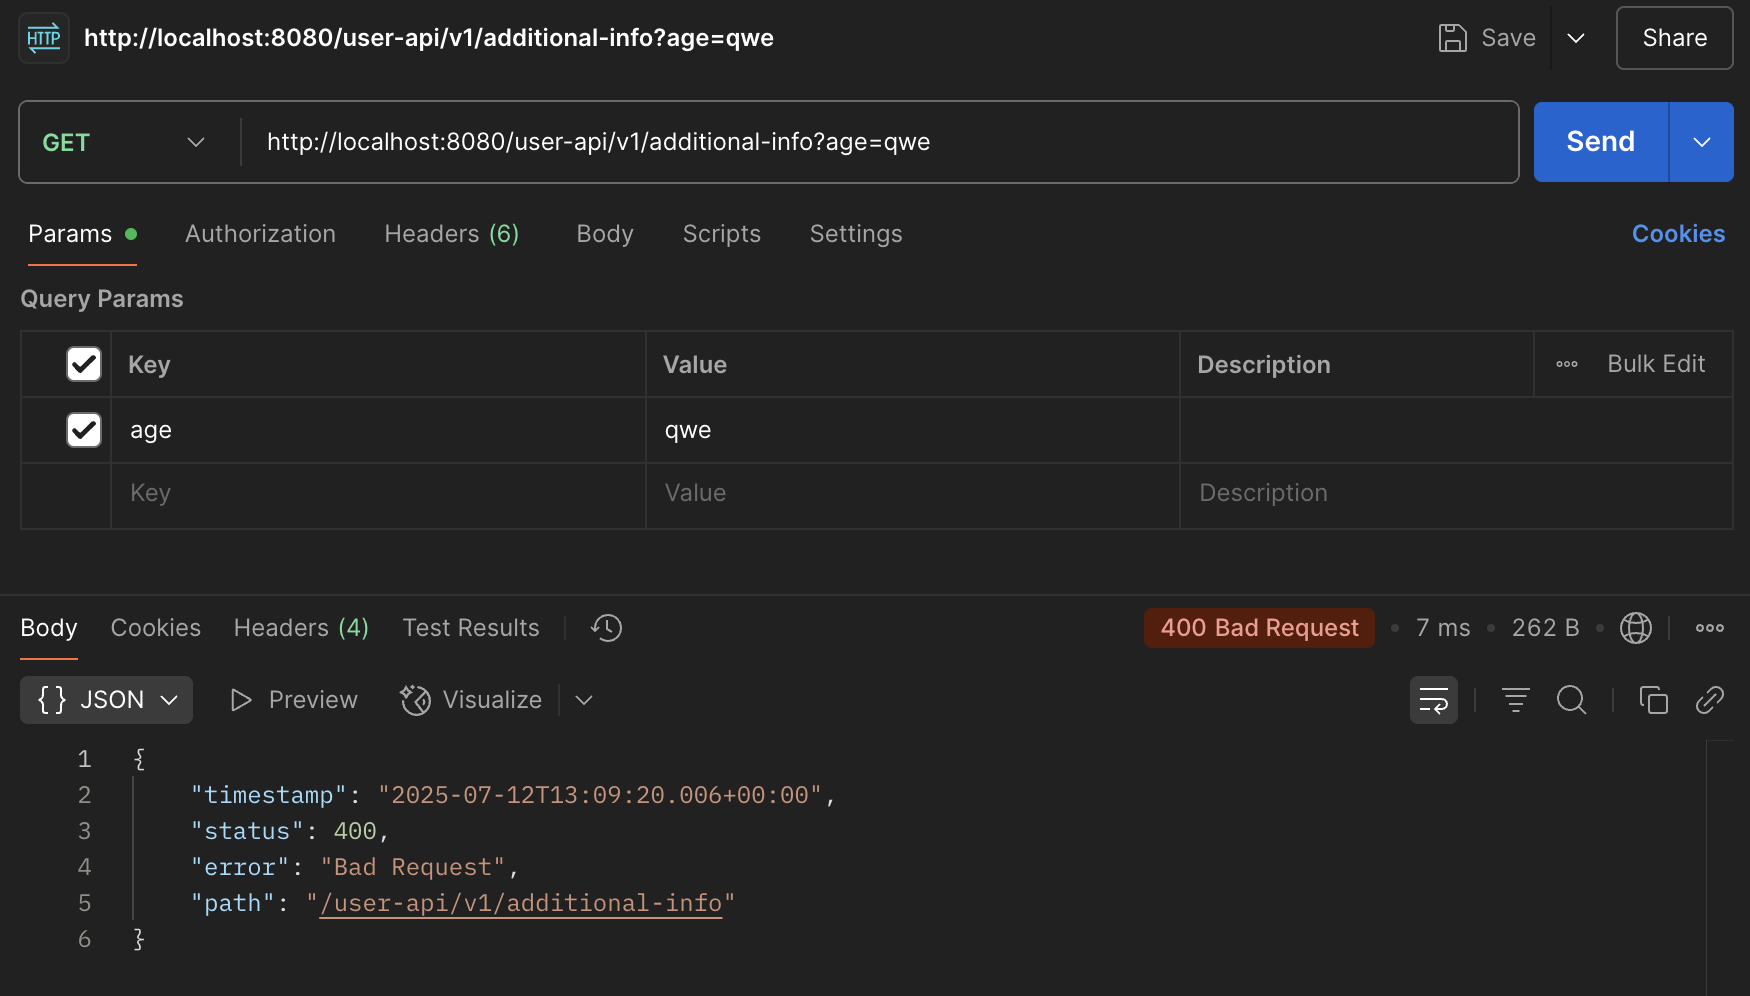
\includegraphics[width=13cm]{resources/10.png}
	\caption{Вывод подробной информации по доходам/расходам/бюджетам}
\end{figure}

\subsection{Вывод подробной информации по доходам/расходам/бюджетам в файл (info-file)}

Команда \texttt{info-file} повторяет работу команды \texttt{info}, однако выводит результат своей работы в файл.

\begin{figure}[H]
	\centering
	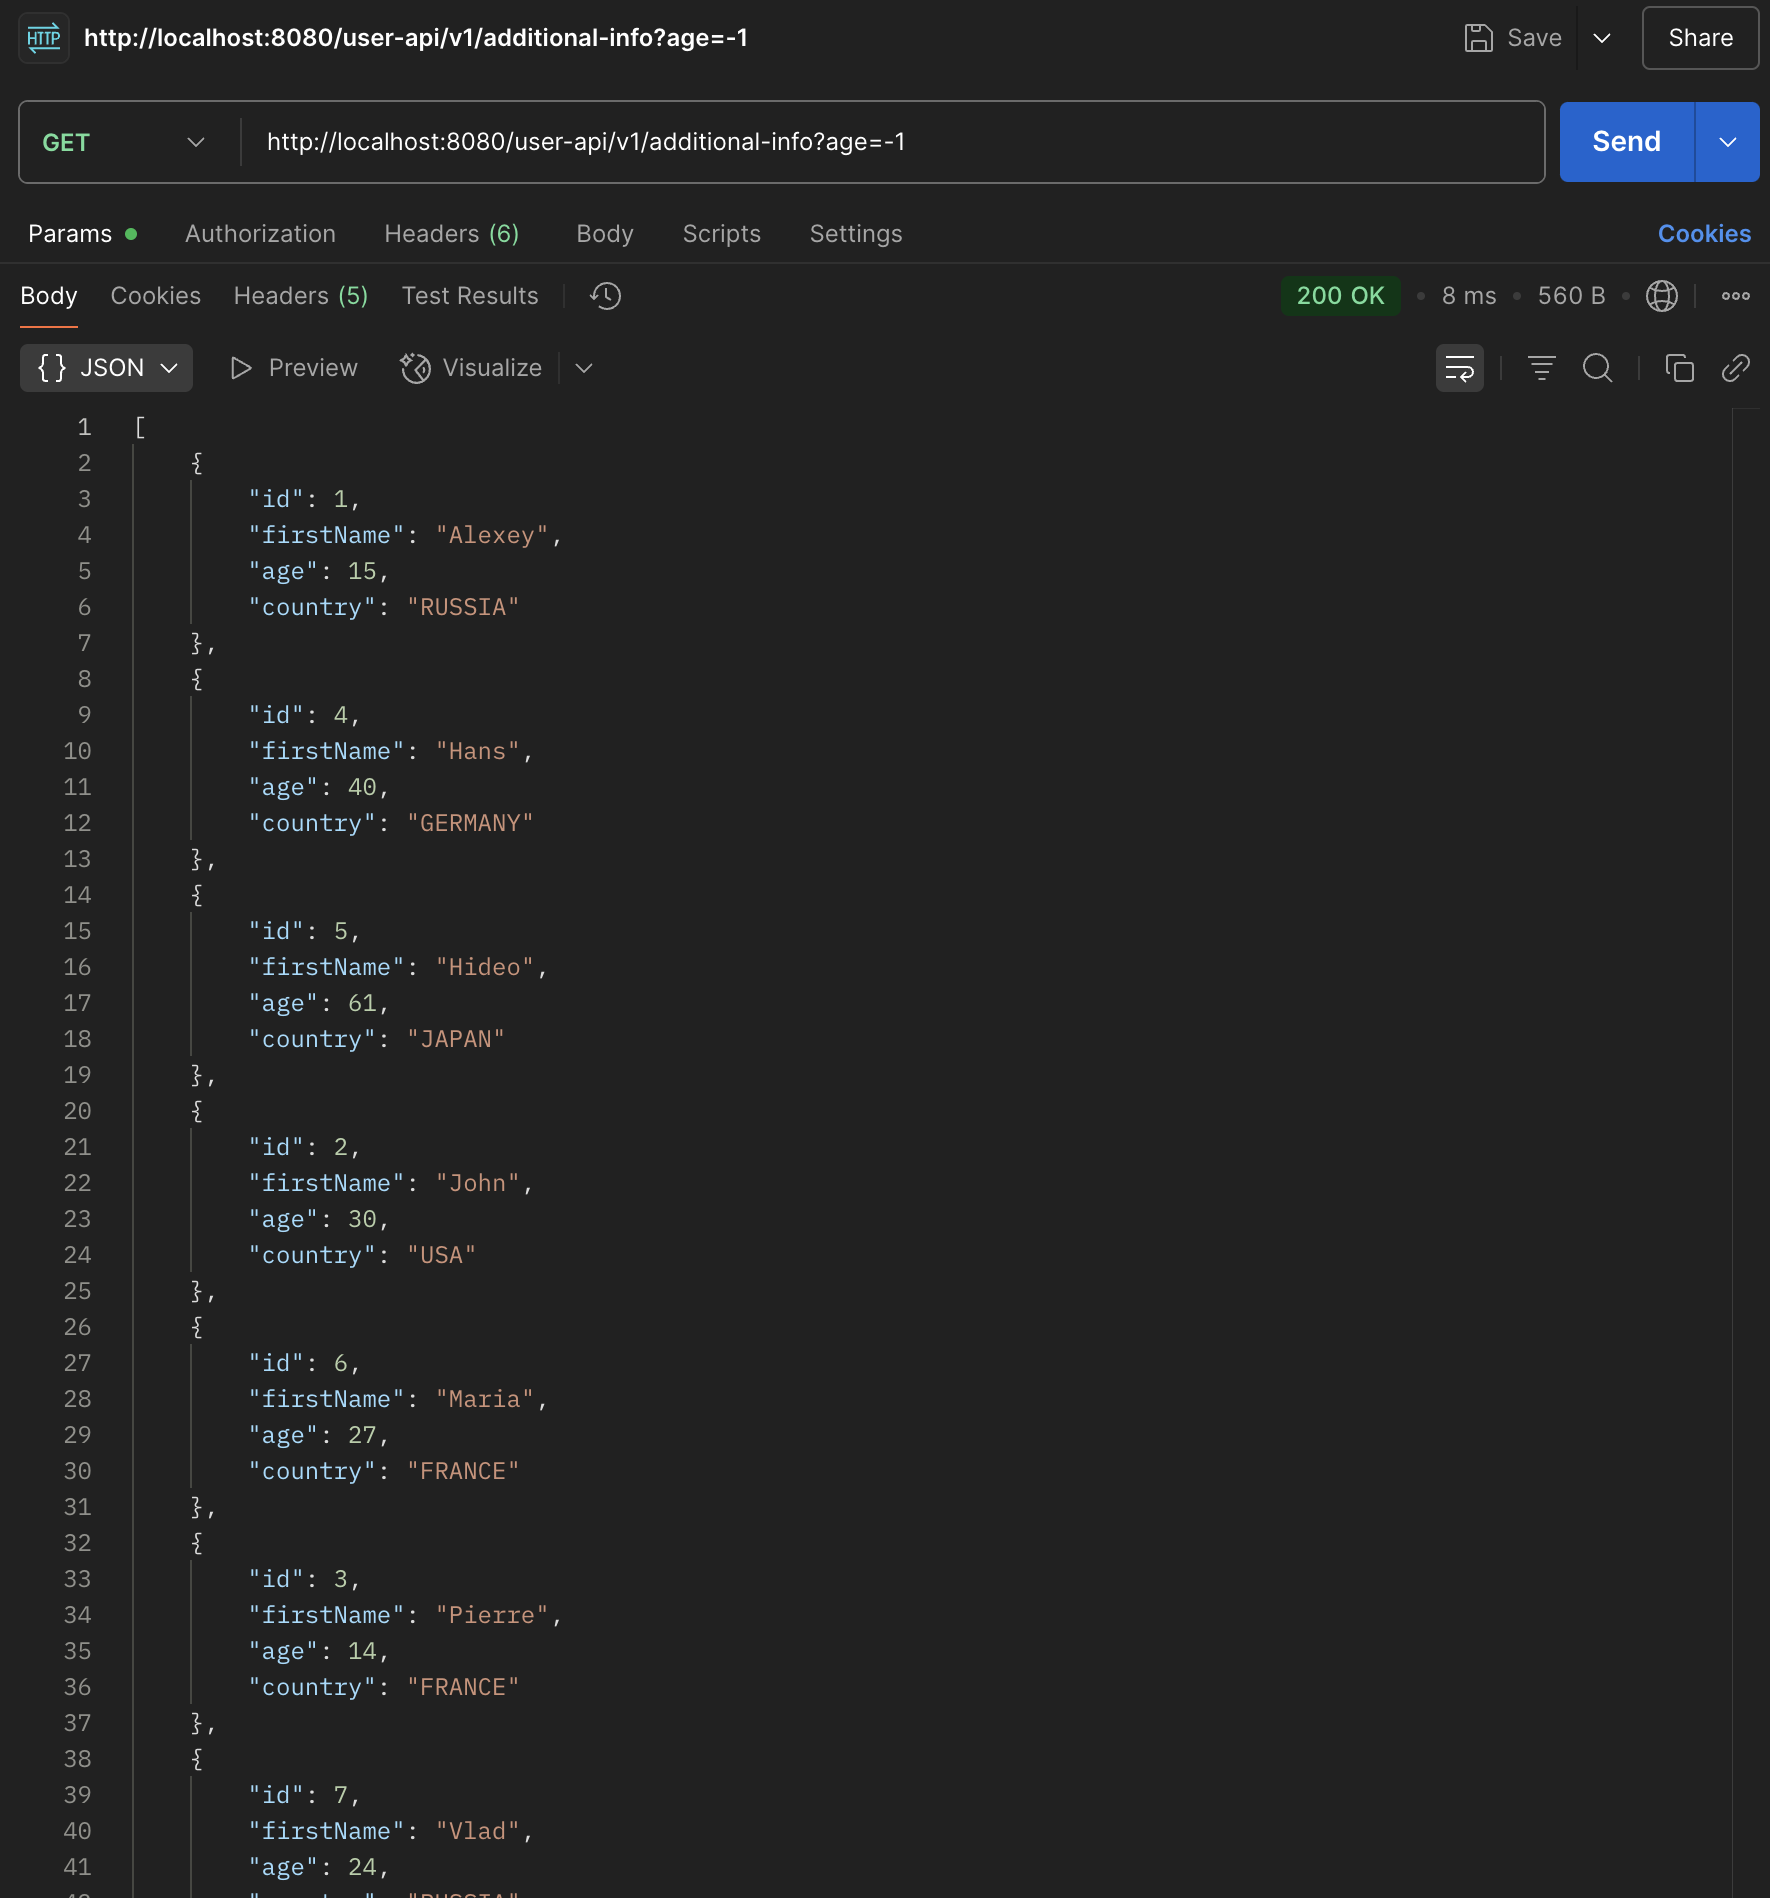
\includegraphics[width=13cm]{resources/11.png}
	\caption{Вывод подробной информации по доходам/расходам/бюджетам в файл}
\end{figure}

Проверим содержимое файла:

\begin{figure}[H]
	\centering
	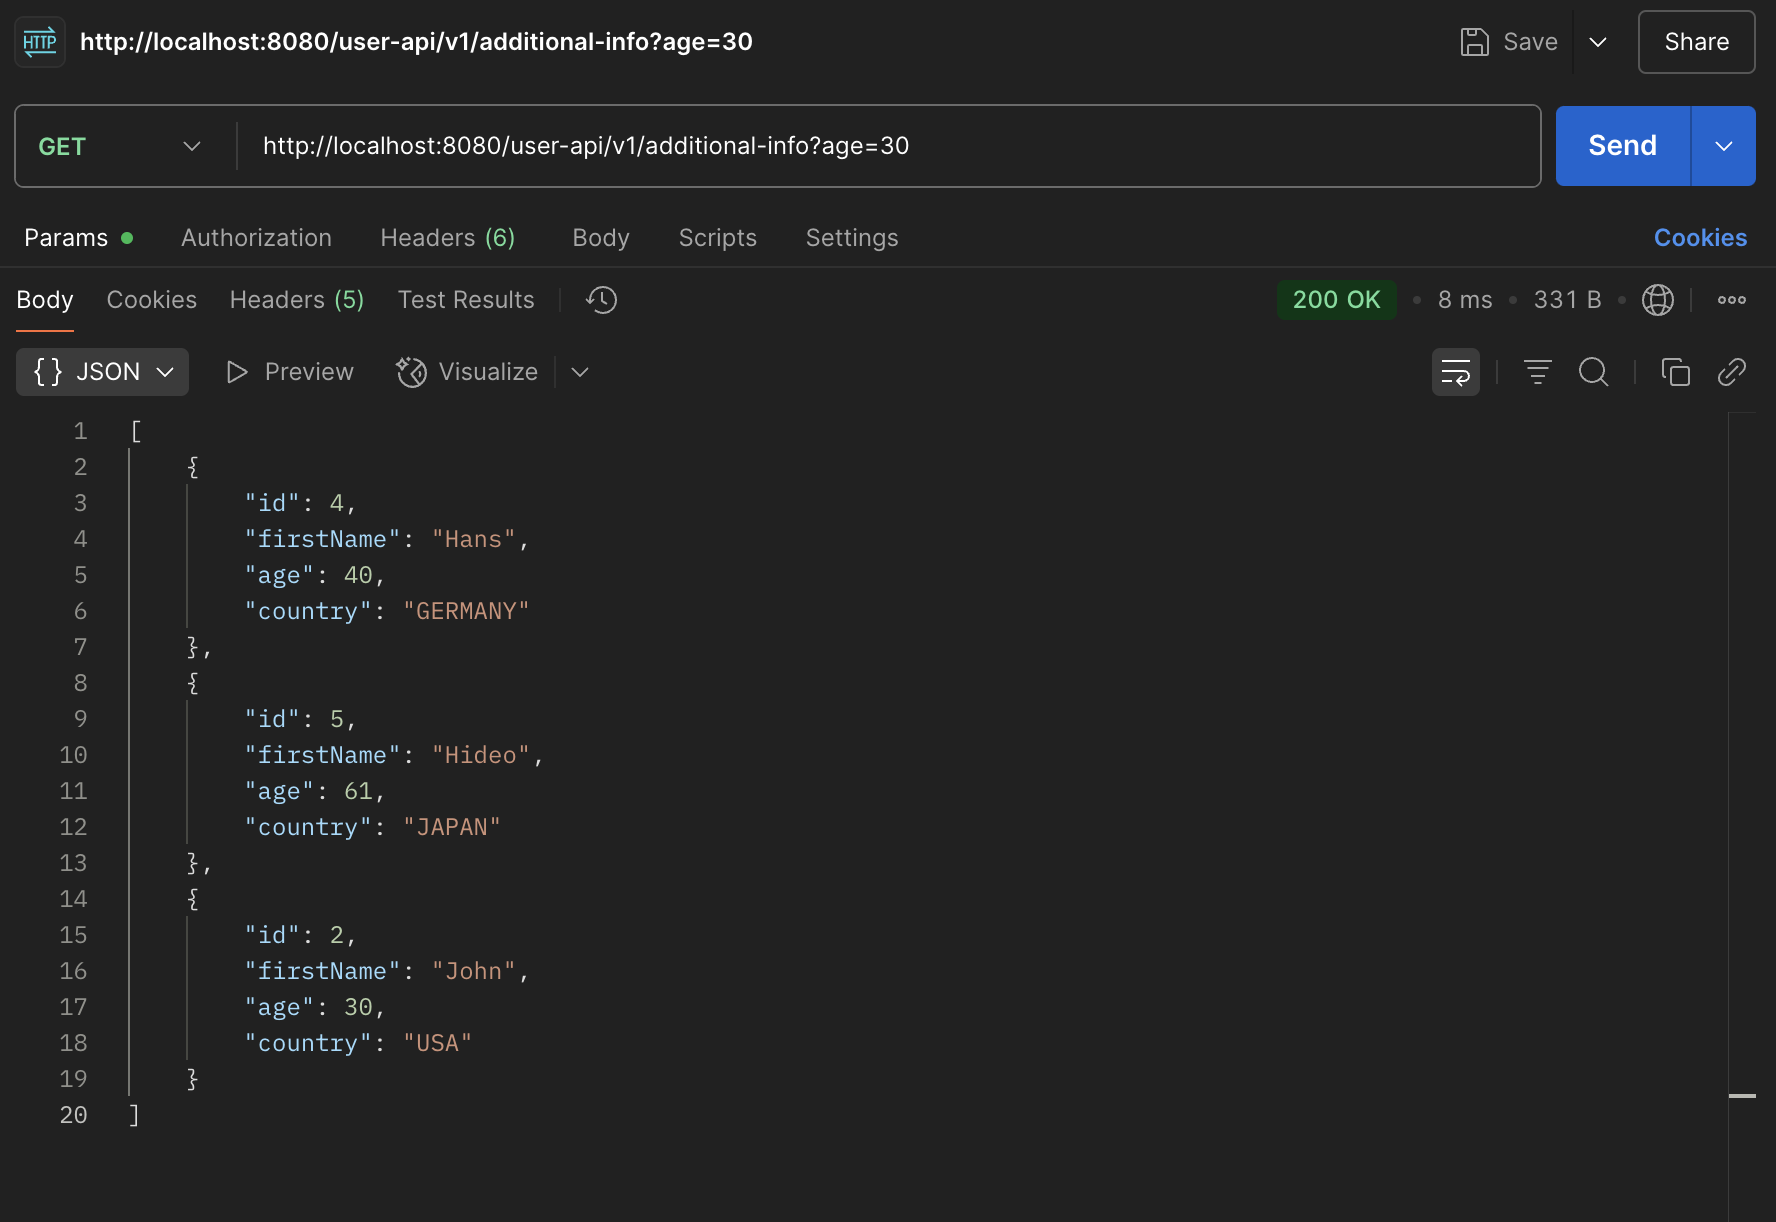
\includegraphics[width=13cm]{resources/12.png}
	\caption{Проверка содержимого файла}
\end{figure}

\subsection{Вывод подробной информации по конкретным категориям (info-certain)}

Команда \texttt{info-certain} выводит подробную информацию о транзакциях по конкретным категориям, которые передаются аргументами. Также она сигнализирует, если категория отсутствует.

Посмотрим ее вывод для трех категорий, две из которых существуют, а одна - нет:

\begin{figure}[H]
	\centering
	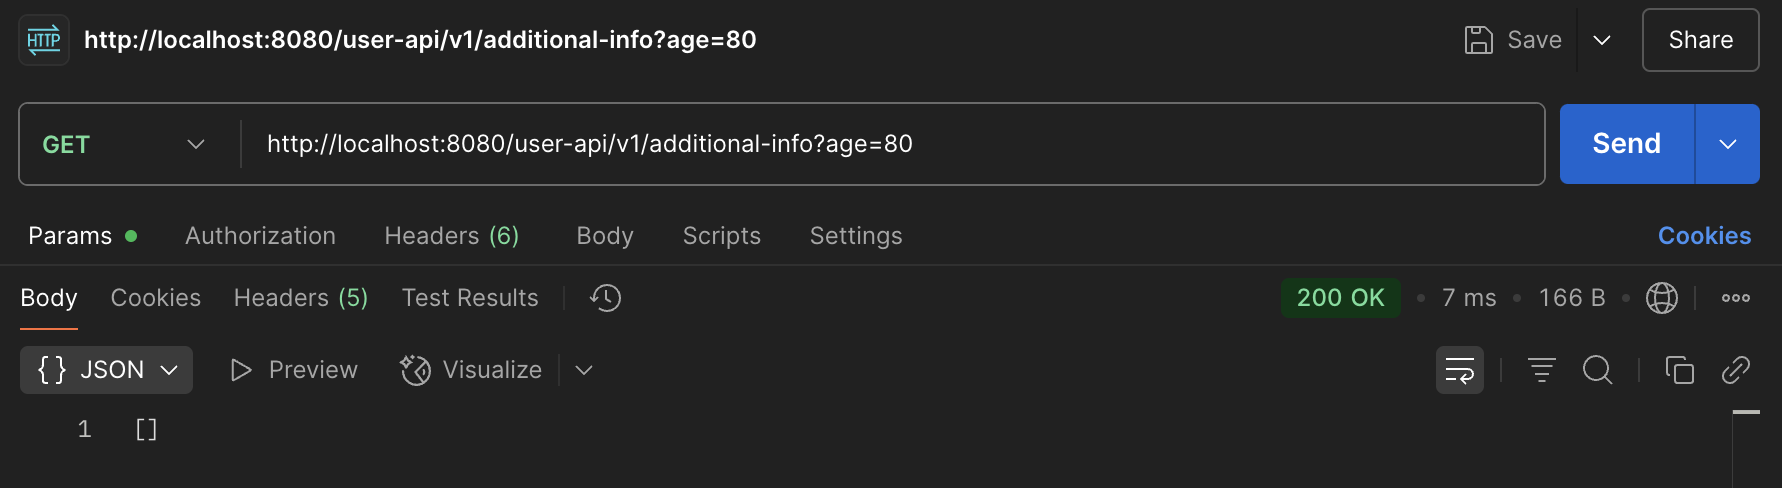
\includegraphics[width=13cm]{resources/13.png}
	\caption{Вывод подробной информации по конкретным категориям}
\end{figure}

\subsection{Выход из программы (exit)}

Наконец, команда \texttt{exit} осуществляет выход из программы:

\begin{figure}[H]
	\centering
	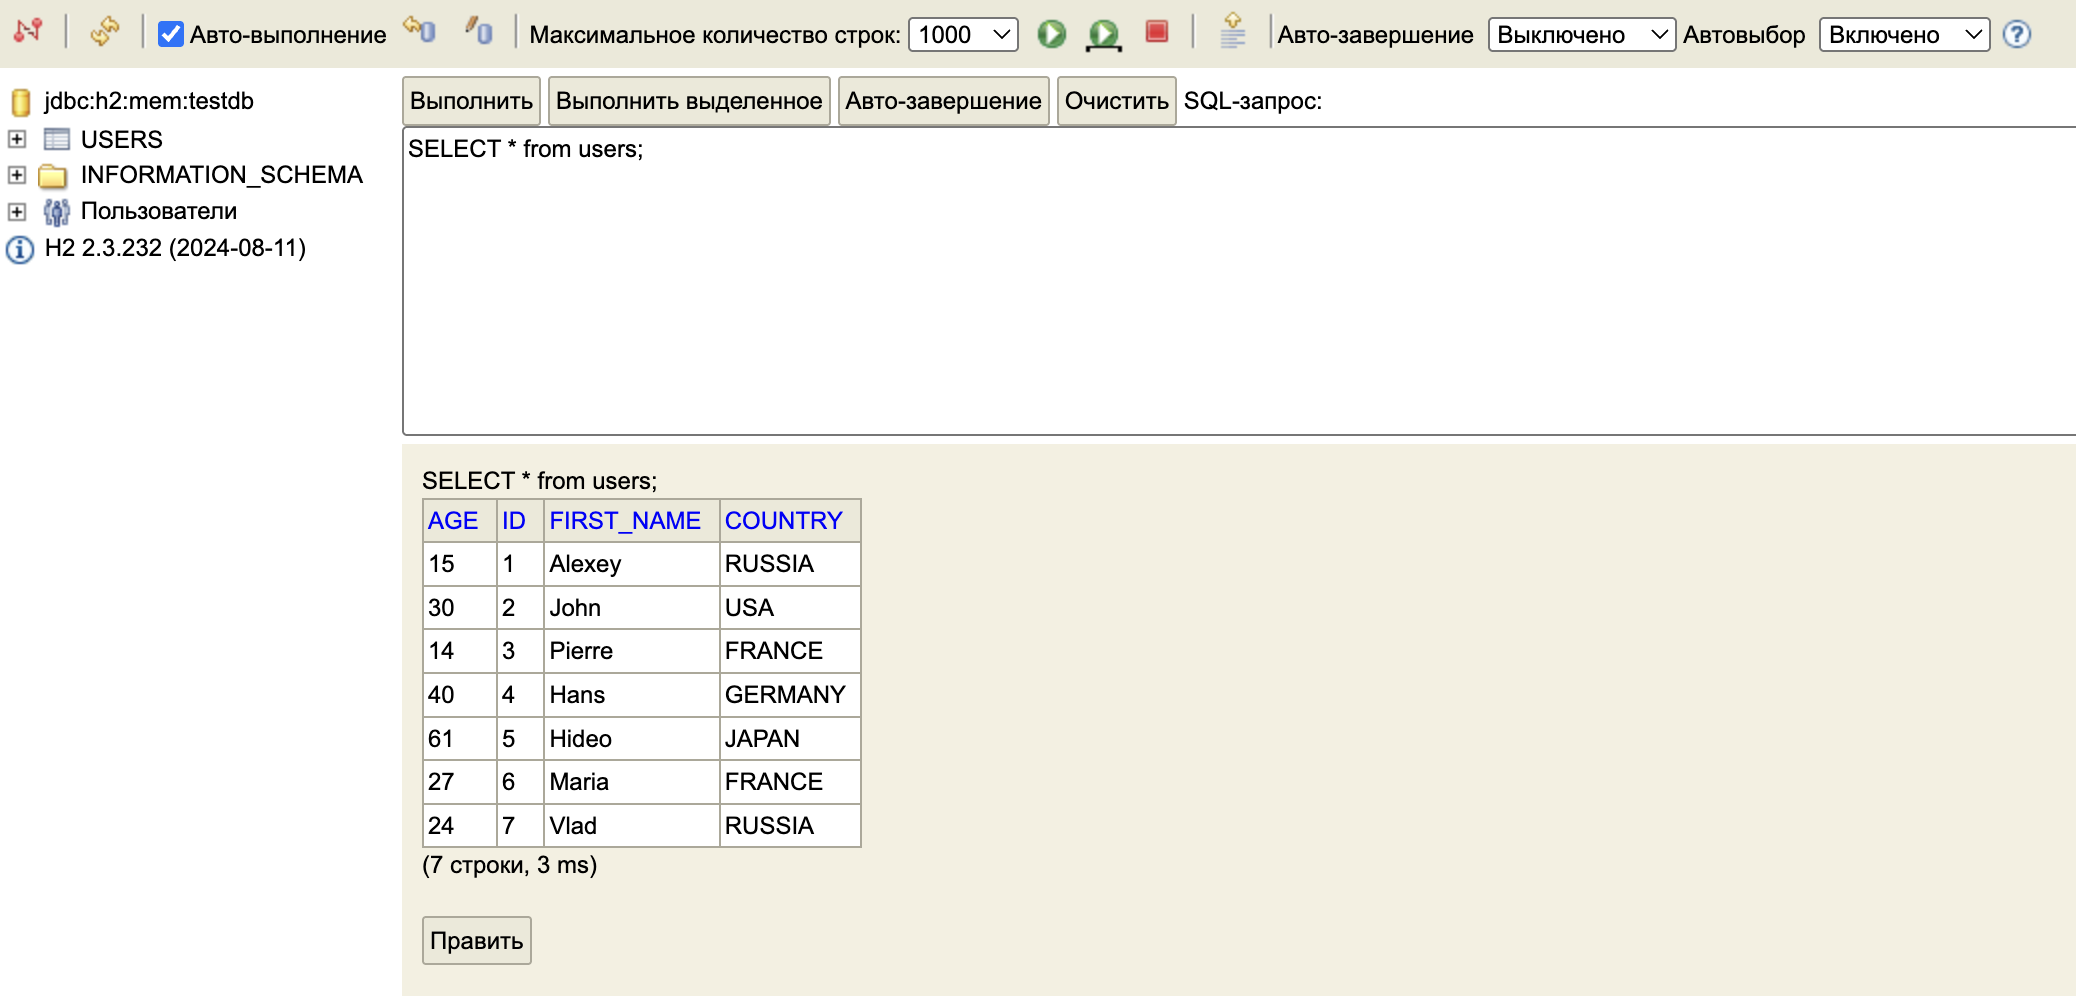
\includegraphics[width=13cm]{resources/14.png}
	\caption{Выход из программы}
\end{figure}

\newpage
\section{Соответствие техническим требованиям}

Ниже будут даны комментарии относительно соответствия программы техническим требованиям.

\subsection{Хранение данных}

\begin{itemize}
	\item Все данные должны храниться в памяти приложения: данное требования реализован с помощью использования БД \texttt{PostgreSQL}.
\end{itemize}

\subsection{Авторизация пользователей}

\begin{itemize}
	\item Реализовать функциональность для авторизации пользователей по логину и паролю. Приложение должно поддерживать несколько пользователей: соответствие данному требованию можно увидеть в работе команд \texttt{login} и \texttt{register}.
\end{itemize}

\subsection{Функционал управления финансами}

\begin{itemize}
	\item Разработать логику для добавления доходов и расходов. Пользователь должен иметь возможность создавать категории для планирования бюджета: соответствие данном требованию можно увидеть в работе команды \texttt{category}.
	\item Предусмотреть функциональность для установления бюджета на каждую категорию расходов: соответствие данному требованию можно увидеть в работе команды \texttt{budget}.
\end{itemize}

\subsection{Работа с кошельком пользователя}

\begin{itemize}
	\item Привязать кошелек к авторизованному пользователю. Кошелек должен хранить информацию о текущих финансах и всех операциях (доходах и расходах): кошельком пользователя является его учетная запись, в ней пользователь создает различные категории, для которых добавляет транзакции. Категории привязаны непосредственно к пользователю, транзакции к конкретной категории.
\end{itemize}

\subsection{Вывод информации}

\begin{itemize}
	\item Реализовать возможность отображения общей суммы доходов и расходов, а также данных по каждой категории: соответствие данному требованию можно увидеть в работе команды \texttt{info}.
	\item Выводить информацию о текущем состоянии бюджета для каждой категории, а также оставшийся лимит: соответствие данному требованию можно увидеть в работе команды \texttt{info}.
	\item Поддерживать вывод информации в терминал или в файл: соответствие данному требованию можно увидеть в работе команды \texttt{info-file}.
\end{itemize}

\subsection{Подсчет доходов и расходов}

\begin{itemize}
	\item Разработать методы, подсчитывающие общие расходы и доходы, а также по категориям соответствие данному требованию можно увидеть в работе команды \texttt{info}.
	\item Поддержать возможность подсчета по нескольким выбранным категориям. Если категория не найдена, уведомлять пользователя: соответствие данному требованию можно увидеть в работе команды \texttt{info-certain}.
\end{itemize}

\subsection{Проверка вводимых данных}

\begin{itemize}
	\item Валидация пользовательского ввода и уведомление о некорректных данных: Для каждой команды проводится тщательная валидация ввода. Для этого используются методы класса \texttt{ValidationUtils}, а также специфические валидации (например, в методе \texttt{pase} класса \texttt{MoneyUtils}).
\end{itemize}

\subsection{Оповещения}

\begin{itemize}
	\item Оповещать пользователя, если превышен лимит бюджета по категории или расходы превысили доходы: в случае, если превышен лимит бюджета по категории или расходы превысили доходы, пользователь будет уведомлен об этом перед вводом очередной команды. Соответствие данному требованию можно, например, увидеть в проверке команды \texttt{transaction} (пункт \texttt{3.6} отчета).
\end{itemize}

\subsection{Сохранение данных}

\begin{itemize}
	\item При выходе из приложения сохранять данные кошелька пользователя в файл:  данное требования реализован с помощью использования БД \texttt{PostgreSQL}.
	\item При авторизации загружать данные кошелька из файла: данное требования реализован с помощью использования БД \texttt{PostgreSQL}.
\end{itemize}

\subsection{Чтение команд пользователя в цикле}

\begin{itemize}
	\item Реализовать цикл для постоянного чтения команд пользователя. Поддержать возможность выхода из приложения: данное требования реализовано с помощью классов команд (пакет \texttt{command}), а также использования паттерна \texttt{Стратегия} (пакет \texttt{handler}).
\end{itemize}

\newpage
\section{Соответствие критериям оценивания}

Ниже будут даны комментарии относительно соответствия программы критериям оценивания.

\subsection{Реализация авторизации пользователей}

Пользователь может зарегистрироваться и войти в систему. Только аутентифицированный пользователь может полноценно работать с программой.

\subsection{Взаимодействие с пользователем}

Взаимодействие с пользователем осуществляется через консоль.

\subsection{Управление доходами и расходами}

В программе реализовано управление доходами и расходами: их добавление, установка бюджета на конкретные категории, вывод отчетов.

\subsection{Работа с кошельком пользователя}

Пользователь может добавлять в свой кошелек категории доходов или расходов, устанавливать бюджет и добавлять транзакции.

\subsection{Вывод информации}

Реализован подробный вывод информации как в консоль, так и в файл.

\subsection{Оповещения пользователя}

Перед вводом команды пользователь оповещается о возможном превышении расходов над доходами, а также о превышении конкретных бюджетов.

\subsection{Сохранение и загрузка данных}

Для сохранения и загрузки данных реализовано взаимодействие с БД \texttt{PostgreSQL}.

\subsection{Чтение команд в цикле}

Команды пользователя считываются в бесконечном цикле, выход из которого происходит после ввода команды \texttt{exit}.

\subsection{Валидация данных}

Вводимые пользователем данные тщательно валидируются как базовыми методами (например, проверка количества аргументов для команды), так и специфическими (например, проверка корректности ввода денежного значения).

\subsection{Дополнительные возможности}

Креативным решением данного приложения предлагаю считать использование паттерна \texttt{Стратегия}, что подчеркивает использование практик чистого кода и принципов \texttt{ООП} и позволяет быстро и удобно добавлять новые команды.

\subsection{Разделение функционала по классам}

Код приложения тщательно разделен на классы и пакеты для удобочитаемости и облегчения поддержки.
\fi

\end{document}